\documentclass[aspectratio=169,usenames,dvipsnames]{beamer}

% fonts
%\usepackage[T1]{fontenc}
%\usepackage[utf8]{inputenc}

%\usefonttheme{professionalfonts} % using non standard fonts for beamer
\usefonttheme{serif} % default family is serif

\usepackage{palatino}
%\usepackage{gfsartemisia}
%\usepackage{theanooldstyle}

\usepackage{euscript}	 % Шрифт Евклид
\usepackage{mathrsfs} % Красивый матшрифт
\usepackage{amssymb}
\usepackage{bm}
\usepackage{calc} % perform arithmetic on the arguments
\usepackage{cancel} % cancelling things
\usepackage{marvosym} % fancy arrow
\usepackage[ruled,vlined]{algorithm2e}
\usepackage{algorithmic}

\definecolor{mygreen}{HTML}{348A41}  % 53945D
\definecolor{myred}{HTML}{B73239} 
\definecolor{myorange}{HTML}{AB5F1F}  % 805129
\definecolor{mypurple}{HTML}{533E8F} 
\definecolor{myblack}{HTML}{4C4848} 
\definecolor{mygrey}{HTML}{F4EDE0} %  F5F1EA

\usepackage{epstopdf}
\usepackage{xcolor}

% adding images
\usepackage{graphicx} 
\usepackage{tcolorbox}

% for ul
\usepackage{soul}

% adding gifs
\usepackage{animate}

% positioning textblocks
\usepackage[absolute, overlay]{textpos} 
\textblockorigin{0mm}{0mm} % start everything near the top-left corner

% Работа с русским языком
\usepackage{cmap}					% поиск в PDF
%\usepackage{mathtext} 				% русские буквы в фомулах
%\usepackage[T2A]{fontenc}			% кодировка
%\usepackage[utf8]{inputenc}			% кодировка исходного текста

% Дополнительная работа с математикой
%\usepackage{amsmath,amsfonts,amssymb,amsthm,mathtools} % AMS
%\usepackage{icomma} % "Умная" запятая: $0,2$ --- число, $0, 2$ --- перечисление

%% Номера формул
%\mathtoolsset{showonlyrefs=true} % Показывать номера только у тех формул, на которые есть \eqref{} в тексте.

% Работа с картинками
\usepackage{graphicx}  % Для вставки рисунков
\graphicspath{{figures/}}  % папки с картинками
\usepackage{wrapfig} % Обтекание рисунков и таблиц текстом

% drawing with tikz
\usepackage{tikz}
\usepackage{hf-tikz}
\usetikzlibrary{arrows}
\usetikzlibrary{shapes}
\usetikzlibrary{plotmarks}

\tikzset{
	treenode/.style = {align=center, inner sep=1.ex, minimum size=1cm,
		font=\sffamily},
	arn_n/.style = {treenode, rectangle, black, draw=black, minimum width = 0.05\textwidth, minimum height = 1 cm},% 
	level distance = 2.5cm,
	level 1/.style={sibling distance=16.cm},
	level 2/.style={sibling distance=8.cm},
	level 3/.style={sibling distance=3.7cm}
}

  \tikzset{
	invisible/.style={opacity=0},
	visible on/.style={alt=#1{}{invisible}},
	alt/.code args={<#1>#2#3}{%
		\alt<#1>{\pgfkeysalso{#2}}{\pgfkeysalso{#3}} % \pgfkeysalso doesn't change the path
	},
}

%% Работа с таблицами
%\usepackage{array,tabularx,tabulary,booktabs} % Дополнительная работа с таблицами
%\usepackage{longtable}  % Длинные таблицы
%\usepackage{multirow} % Слияние строк в таблице
%\renewcommand{\arraystretch}{1.3} %The height of each row is set to 1.5 relative to its default height. 

% Two ways of getting rid of total slides number

%\setbeamertemplate{footline}
%    {\begin{beamercolorbox}[sep=1ex]{author in head/foot}
%      \rlap{\textit{\insertshorttitle}}\hfill\insertauthor\hfill\llap{\insertframenumber}%
%      \end{beamercolorbox}%
%}

\makeatletter
\setbeamertemplate{footline}
{
	\leavevmode%
	\hbox{%
		\begin{beamercolorbox}[wd=.333333\paperwidth,ht=2.25ex,dp=1ex,center]{author in head/foot}%
			\usebeamerfont{author in head/foot}\insertshortauthor~~\beamer@ifempty{\insertshortinstitute}{}{\insertshortinstitute}
%            {(\insertshortinstitute)}
		\end{beamercolorbox}%
		\begin{beamercolorbox}[wd=.333333\paperwidth,ht=2.25ex,dp=1ex,center]{title in head/foot}%
			\usebeamerfont{title in head/foot}\insertshorttitle
		\end{beamercolorbox}%
		\begin{beamercolorbox}[wd=.333333\paperwidth,ht=2.25ex,dp=1ex,right]{date in head/foot}%
			\usebeamerfont{date in head/foot}\insertshortdate\hspace*{2em}
			\insertframenumber/\inserttotalframenumber\hspace*{2ex} 
	\end{beamercolorbox}}%
	\vskip0pt%
}
\makeatother

% Beamer presentation style
\mode<presentation> {
	\usetheme{Pittsburgh}
	\usecolortheme{dove}
	%\setbeamertemplate{footline} % To remove the footer line in all slides uncomment this line
	%\setbeamertemplate{footline}[page number] % To replace the footer line in all slides with a simple slide count uncomment this line
	%\setbeamertemplate{navigation symbols}{} % To remove the navigation symbols from the bottom of all slides uncomment this line
	
	%	\setbeamercolor{frametitle}{fg=white,bg=greyone}
	%	\setbeamercolor{titlelike}{parent=palette quaternary}
	
	%	\setbeamertemplate{frametitle}
	%	{
	%		\begin{textblock*}{\hsize}(.75\hsize,0.05\vsize)
	%			\begin{tcolorbox}[colframe=white, colback=mygrey, width=0.33\hsize,
	%				arc=2.mm, boxsep=2mm,
	%				box align=center,
	%				halign=center,
	%				valign=center,
	%				]
	%				\insertframetitle
	%			\end{tcolorbox}
	%		\end{textblock*}
	%	}
}

%% custom title
%\newcommand{\myframetitle}[3]{
%	\begin{textblock*}{\hsize}(#1,0.05\vsize)
%		\begin{tcolorbox}[colframe=white, colback=mygrey, width=#2,
%			arc=2.mm, boxsep=2mm,
%			box align=center,
%			halign=center,
%			valign=center,
%			]
%			\Large
%			#3
%		\end{tcolorbox}
%	\end{textblock*}
%}

% custom title
\newcommand{\myframetitle}[3]{
	\begin{textblock*}{#1}(#2,0.05\vsize)
		\begin{tcolorbox}[colframe=white, colback=mygrey, width=#1,
			arc=2.mm, boxsep=2mm,
			box align=center,
			halign=center,
			valign=center,
			]
			\Large
			\centering
			#3
		\end{tcolorbox}
	\end{textblock*}
}

% custom subtitle
\newcommand{\myframesubtitle}[2]{
	
	\begin{textblock*}{5cm}(#1,0.123\vsize)
		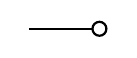
\begin{tikzpicture}
		\draw[thick,-o,black] (0.,0.) -- (1.0,0.);
		\end{tikzpicture}
	\end{textblock*}
	
	\begin{textblock*}{0.5\hsize}(#1+0.075\paperwidth,0.1\vsize)
		\normalsize
		\vspace{0.6mm}
		%		\centering
		#2
	\end{textblock*}
}

% new color for the bullet/subbullet
\newcommand{\mybullet}{$\textcolor{myblack}{\bullet}$}
\newcommand{\mysubbullet}{$\textcolor{myblack}{\circ}$}
\newcommand{\ev}{\mathbb{E}_{\text{p}(\bm x,y)}}
\newcommand{\pluseq}{\mathrel{+}=}

\newcommand{\beginbackup}{
   \newcounter{framenumbervorappendix}
   \setcounter{framenumbervorappendix}{\value{framenumber}}
}
\newcommand{\backupend}{
   \addtocounter{framenumbervorappendix}{-\value{framenumber}}
   \addtocounter{framenumber}{\value{framenumbervorappendix}} 
}

%----------------------------------------------------------------------------------------
%	TITLE PAGE
%----------------------------------------------------------------------------------------

\author[Sergey Korpachev]{Sergey Korpachev}%
%\author[Sergey Korpachev]{Sergey Korpachev\inst{1, 2} on behalf of Dépôt}%
\author[Sergey Korpachev]{Sergey Korpachev on behalf of Dépôt}
\institute[]{
%\institute[MIPT, LPI]{
%	\newline
%	\inst{1} {Moscow Institute of Physics and Technology}\\
%	\vspace{1mm}
%	\inst{2} {Lebedev Physical Institute of the Russian Academy of Sciences}\\
}
%\titlegraphic{
%	%\vspace{-.5cm}
%	%\hspace{1cm}
%	
\includegraphics[width=2.5cm]{mipt_logo.png}\hspace*{0.1cm}
%	
\includegraphics[width=1.5cm]{images/newLogoLPI.png}\hspace*{0.6cm}
%}

\title[Machine Learning (GitHub: SergeyKorpachev)]{}
%\date[\today]{}
\date[April 10, 2025]{}

%------------------------------------------------

\begin{document}

\begin{frame}
\centering
\huge

%\vspace{-0.3\paperheight}
\begin{tcolorbox}[colframe=white, colback=mygrey, width=0.45\paperwidth,
	arc=2.mm, boxsep=2mm,
	box align=center,
	halign=center,
	valign=center,
	]
	\Large
	Machine Learning: short introduction\\
    (trees and ANN),\\
    part 2
\end{tcolorbox}

\vspace{0.1\paperheight}
\centering
\large
\insertauthor\\

\scriptsize
\vspace{0.03\paperheight}
\hspace{0.17\paperwidth}
\insertinstitute

\vfill
\inserttitlegraphic
\transfade[duration=.4]
\end{frame}

%%------------------------------------------------
%------------------------------------------------
\section{Outline}
%------------------------------------------------
%------------------------------------------------

\begin{frame}[t]
\myframetitle{0.2\paperwidth}{0.04\paperwidth}{\insertsection}

\vspace{0.20\paperheight}
\begin{itemize}
    \centering
	\itemsep1.2ex
	\setbeamertemplate{items}{\mybullet}
	\item Machine learning (ML)
	\item Data
	\item Features in ML
	\item ML pipeline
	\item Linear model
	\item Decision tree
	\item Neural network
 	\item Summary
\end{itemize}

\transfade[duration=.4]
\end{frame}

%------------------------------------------------
%------------------------------------------------
\section{Decision tree}
%------------------------------------------------
%------------------------------------------------

\begin{frame}[plain]
\centering
\huge

%\begin{textblock*}{0.3\paperwidth}(0.25\paperwidth,0.3\paperheight)
\centering
\vspace{0.1\paperheight}
\begin{tcolorbox}[colframe=white, colback=mygrey, width=0.4\paperwidth,
	arc=2.mm, boxsep=2mm,
	box align=center,
	halign=center,
	valign=center,
	]
	\insertsection
\end{tcolorbox}

%\end{textblock*}

\transfade[duration=.4]
\end{frame}

%------------------------------------------------

\subsection{motivation}
\begin{frame}

\myframetitle{0.27\paperwidth}{0.04\paperwidth}{\insertsection}
\myframesubtitle{0.29\paperwidth}{\insertsubsection}

\centering
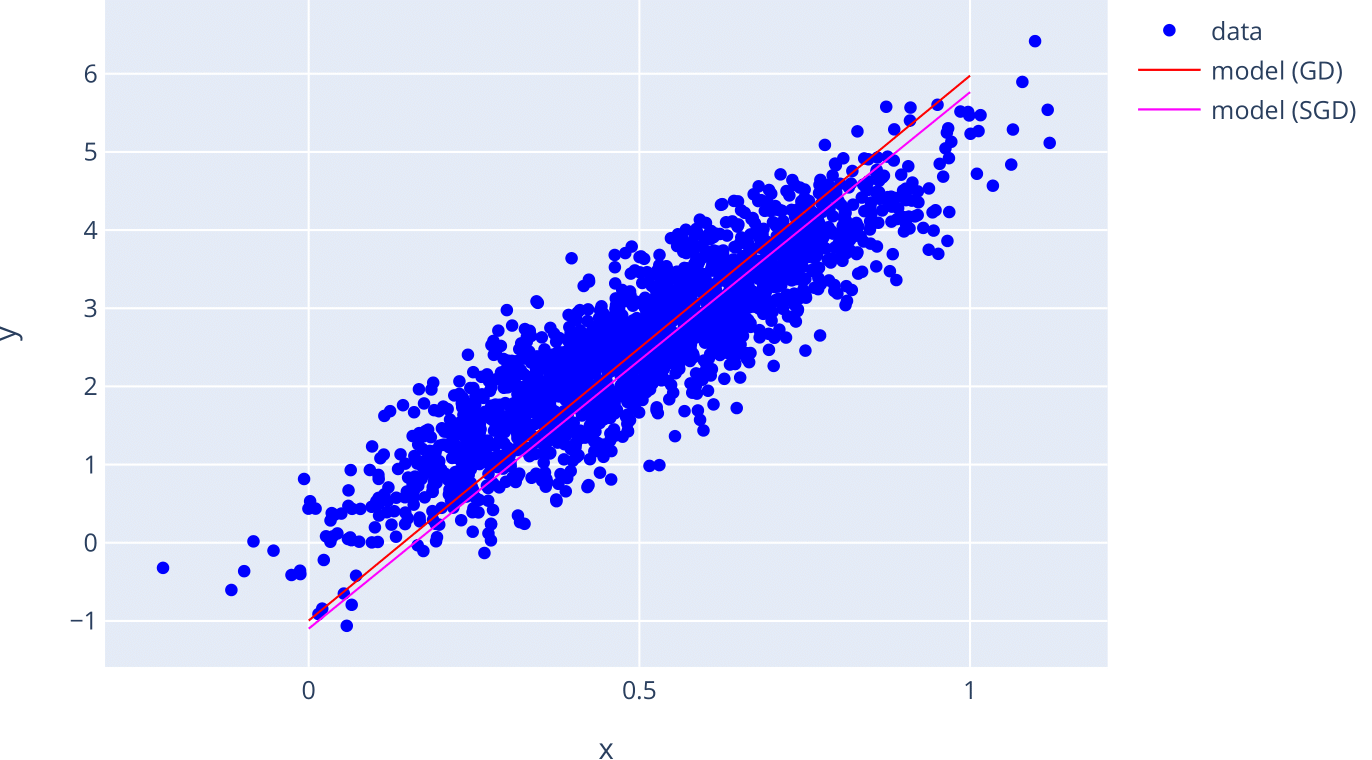
\includegraphics[width=0.3\textwidth]{data+fit.png}
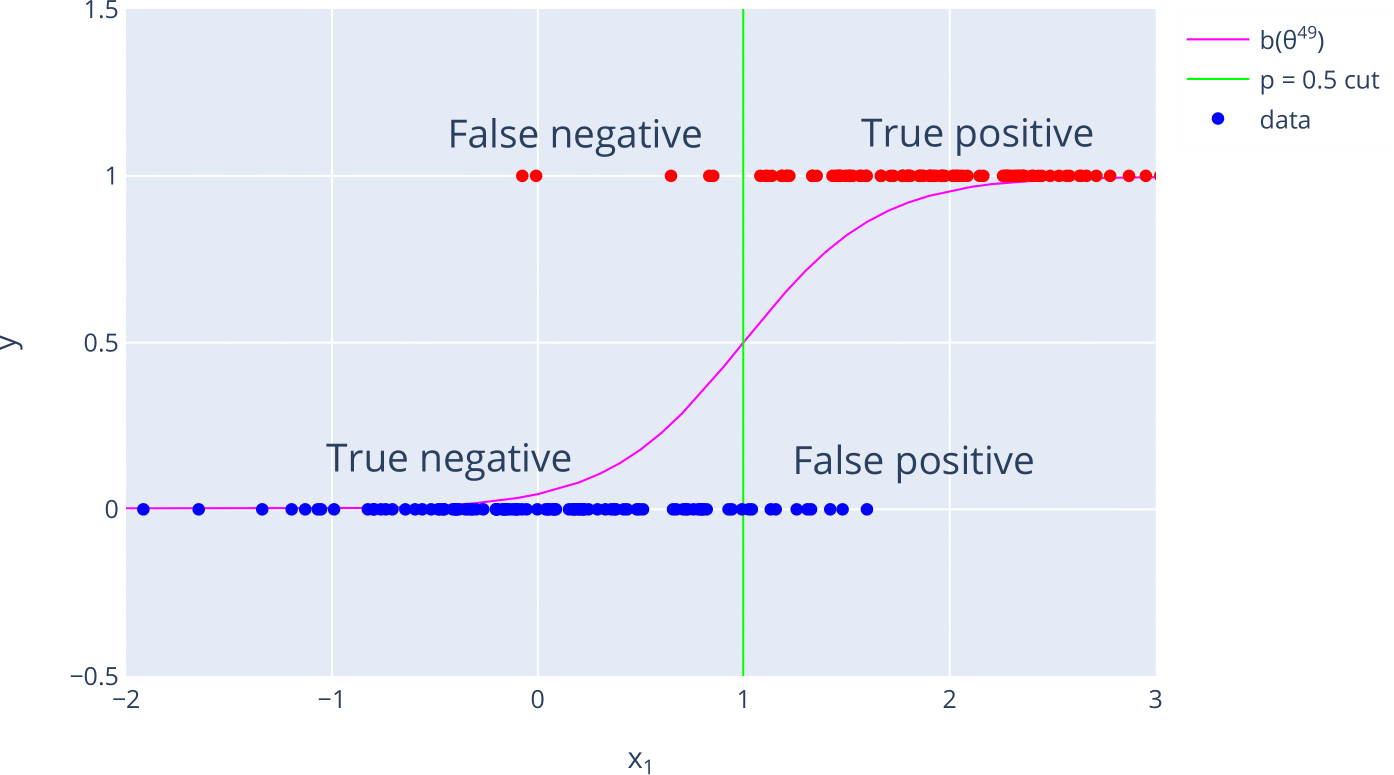
\includegraphics[width=0.3\textwidth]{class_confusions.png}
\only<2->{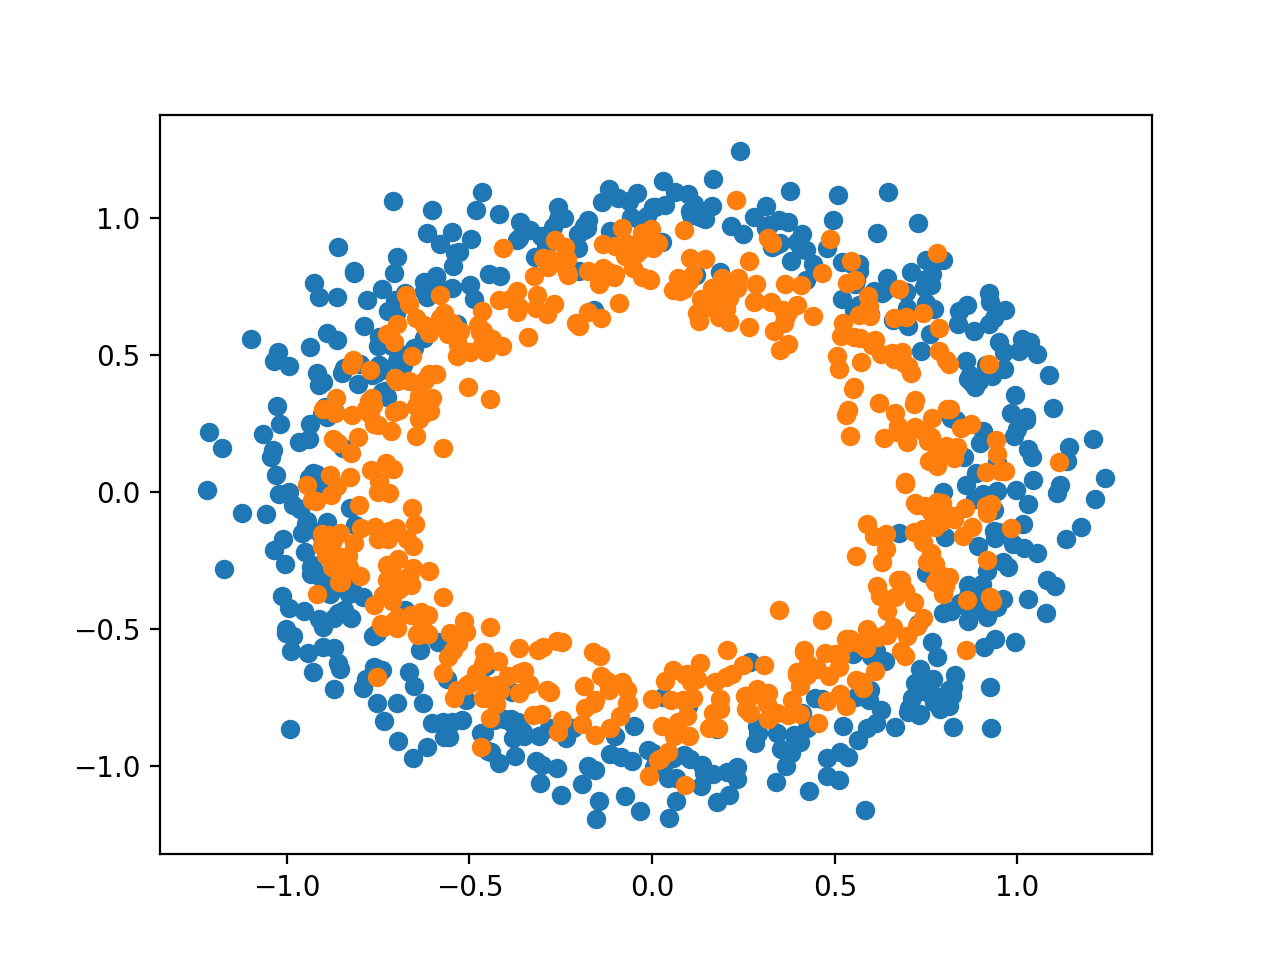
\includegraphics[width=0.25\textwidth]{circles}}

\begin{textblock*}{0.9\paperwidth}(0.05\paperwidth, 0.6\paperheight)
\begin{itemize}
	\itemsep0.8ex
	\footnotesize
	\setbeamertemplate{items}{\mybullet}
	\item In the previous part we explored linear models:
	\begin{itemize}
		\footnotesize
		\setbeamertemplate{items}{\textcolor{Gray}{\MVRightArrow}}
		\item nicely describe linear correlations
		\item fast and easy to train
%		\item performing well with large number of samples/features
	\end{itemize}
	\item<2-> However, they are poor in modelling non-linearities
	\item<2-> Additional heuristics might be applied (e.g. polynomial features) but are ad-hoc
\end{itemize}

\begin{textblock*}{0.3\paperwidth}(0.67\paperwidth, 0.7\paperheight)
	\footnotesize
	\only<3->{\centering \textcolor{myorange}{Is there a more general way to describe non-linearities?}}
\end{textblock*}	

\end{textblock*}
\end{frame}

%------------------------------------------------

\begin{frame}\myframetitle{0.27\paperwidth}{0.04\paperwidth}{\insertsection}
\myframesubtitle{0.29\paperwidth}{\insertsubsection}
\vspace{0.25\textheight}
\begin{itemize}
    \item[\mybullet]  What is the simplest way to approximate a function?
    \item[\mybullet] Using \textbf{piecewise linear function}
\end{itemize}
   \begin{columns}
   \column{0.5\linewidth}
    \begin{figure}
        \centering
        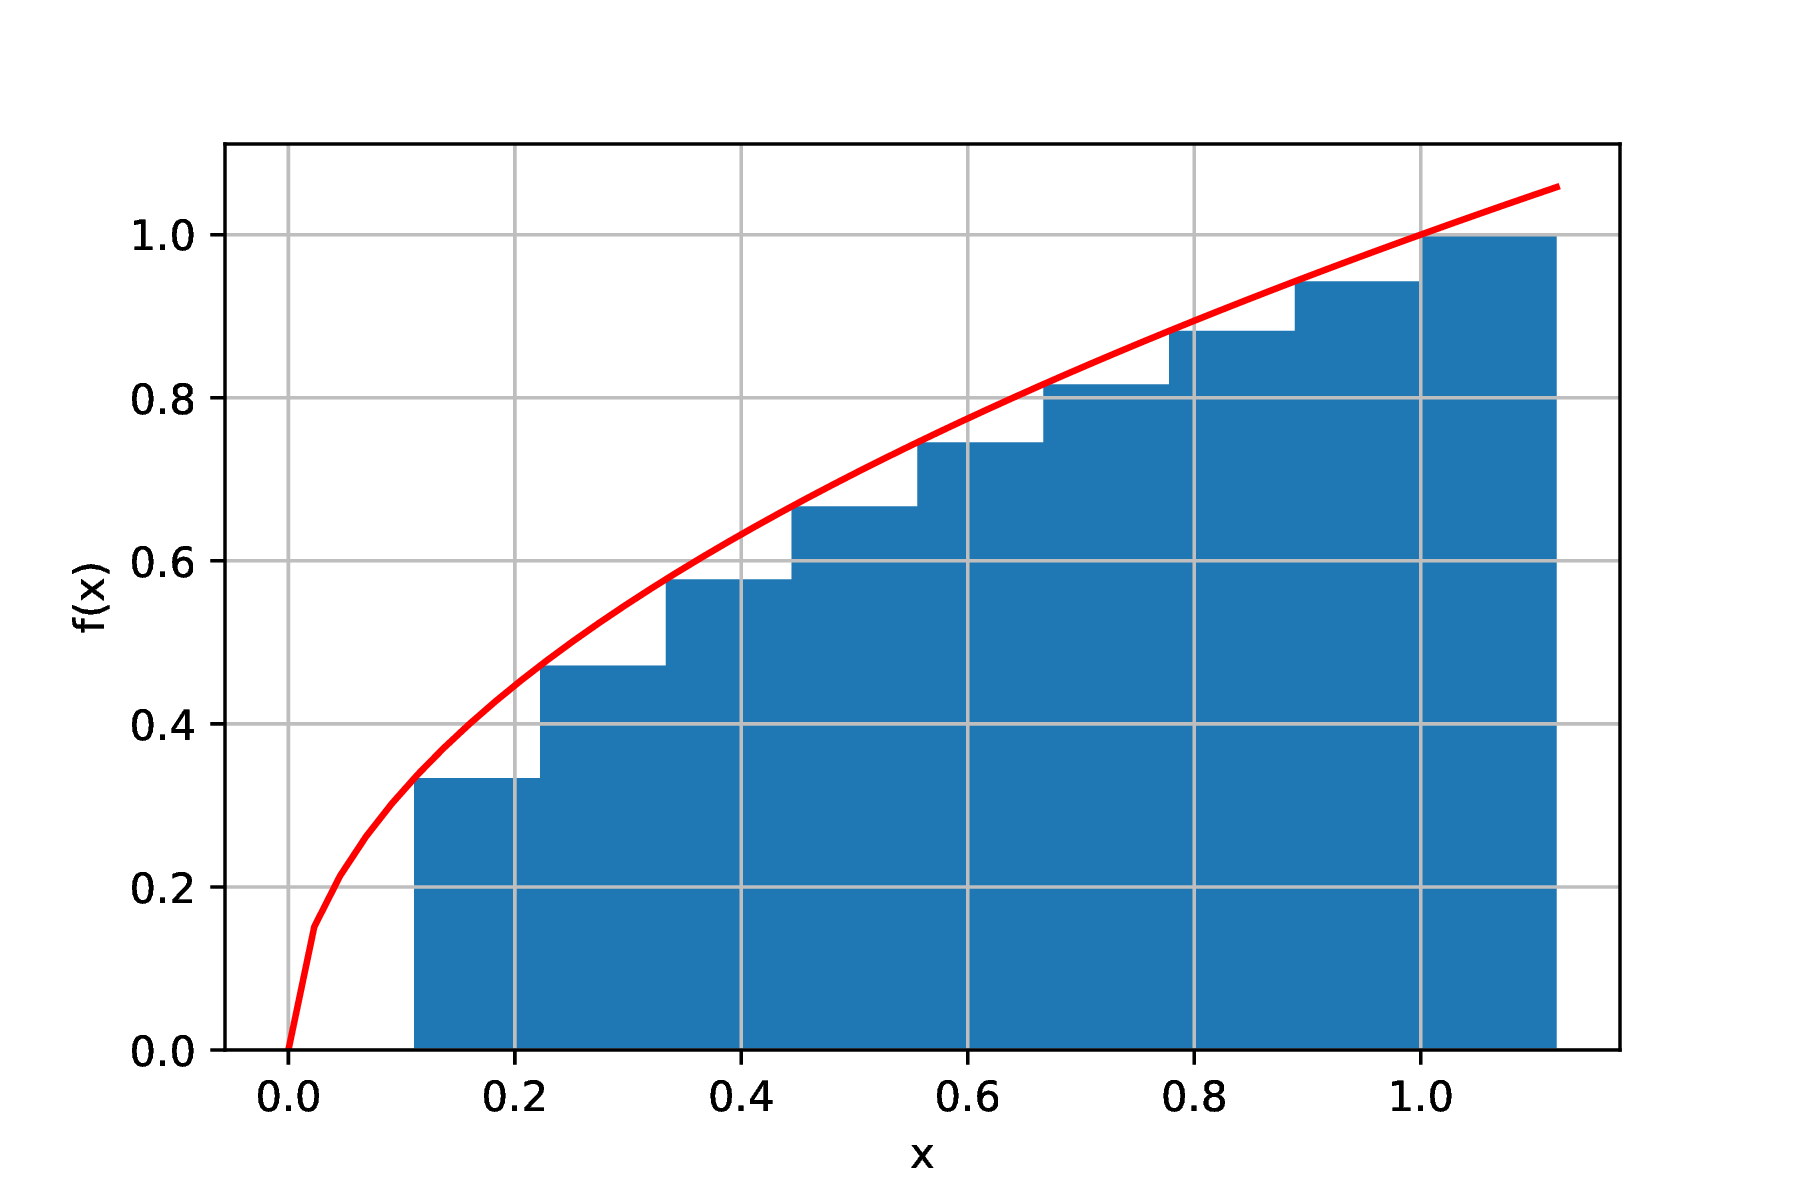
\includegraphics[width=1\linewidth]{plot.png}
    \end{figure}
    \column{0.5\linewidth}
    \begin{equation*}
       f(x) = \begin{cases}
        0 , &x < 0.12 \\
        0.35, &0.12 \leq x < 0.22\\
        0.47, &0.22 \leq x < 0.36\\
        \dots
        \end{cases}
    \end{equation*}
   \end{columns}
   
\end{frame}

%------------------------------------------------

\subsection{intuition}

\begin{frame}

\myframetitle{0.27\paperwidth}{0.04\paperwidth}{\insertsection}
\myframesubtitle{0.29\paperwidth}{\insertsubsection}

\vspace{0.25\paperheight}

\begin{textblock*}{.6\paperwidth}(0.05\paperwidth, 0.2\paperheight)
\begin{itemize}
	\item[\mybullet] What is the simplest way to categorize things?
	\item[\mybullet] Ask \textbf{yes/no questions}
\end{itemize}
\end{textblock*}

\vspace{0.05\paperheight}
\only<1>{
\begin{figure}
	\centering
	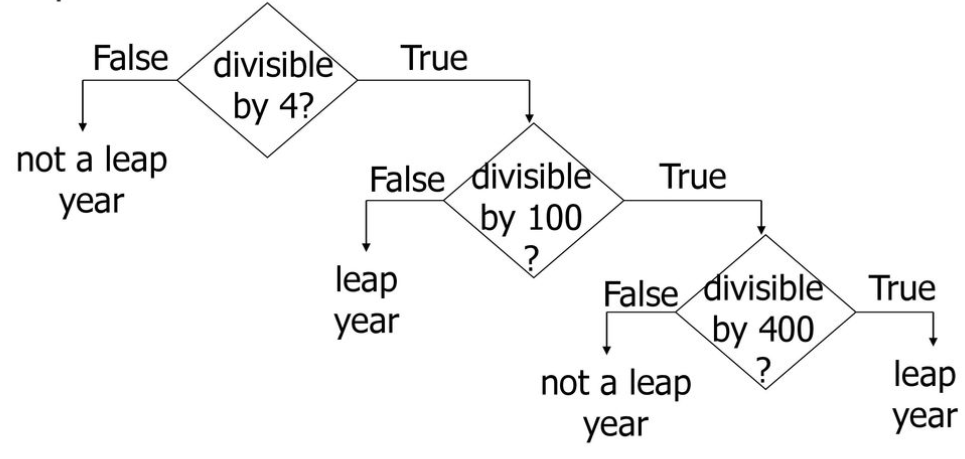
\includegraphics[width=0.6\textwidth]{leapyear.png}
\end{figure}
}

\only<2->{
\begin{figure}
	\centering
	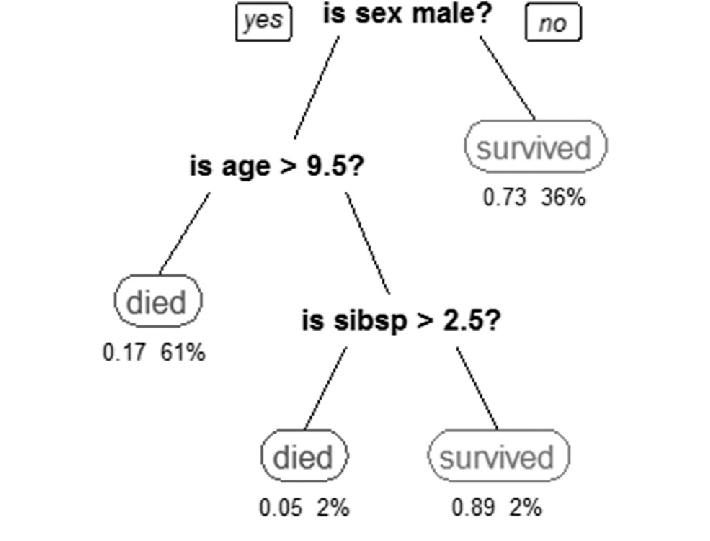
\includegraphics[width=0.35\textwidth]{titanic.png}
\end{figure}
}

\begin{textblock*}{.5\paperheight}(0.7\paperwidth, 0.6\paperheight)
	\only<3->{\textcolor{myorange}{Can we mathematically formulate this?}}
\end{textblock*}

%\vfill
%source: https://slideplayer.com/slide/12812756/
\end{frame}

%------------------------------------------------

\subsection{algorithm}
\begin{frame}
\myframetitle{0.27\paperwidth}{0.04\paperwidth}{\insertsection}
\myframesubtitle{0.29\paperwidth}{\insertsubsection}

\vspace{0.2\paperheight}
\begin{columns}
\column{0.55\linewidth}
\begin{algorithm}[H]
\begin{algorithmic}[1]
\small
\vspace{0.5ex}
\STATE Initialize: hyperparameters, leaf set = $\{\text{X}_\text{train}\}$
\vspace{0.5ex}
\WHILE{not stopping criteria}
\vspace{0.2ex}
\STATE leaf to split = Choose(leaf set)
\vspace{0.2ex}
\STATE left leaf, right leaf = Split(leaf to split)
\vspace{0.2ex}
\STATE Add left leaf, right leaf to leaf set
\STATE Remove leaf to split from leaf set
\vspace{0.2ex}
\ENDWHILE
\end{algorithmic}
\caption{Decision tree}
\label{alg:seq}
\end{algorithm}
\column{0.45\linewidth}
\centering
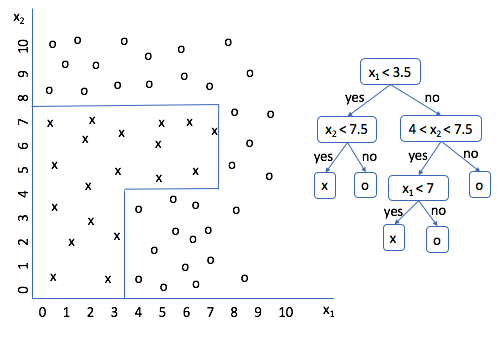
\includegraphics[width=1.\textwidth]{class_tree_scheme.png}
\end{columns}

\end{frame}

%------------------------------------------------

\subsection{split criteria}

\begin{frame}
\myframetitle{0.27\paperwidth}{0.04\paperwidth}{\insertsection}
\myframesubtitle{0.29\paperwidth}{\insertsubsection}

\vspace{0.2\paperheight}
\begin{columns}
	\begin{column}{0.6\textwidth}
		\begin{itemize}
%			\itemsep0.8ex
			\small
			\setbeamertemplate{items}{\mybullet}
			\item Suppose there is a classification problem
			\item So we want to separate one class from the other by constructing \textbf{decision boundary}
			\item And using decision tree algorithm described earlier
			\item To do that we need to start splitting on features
			\item Which \textbf{split} is the best?
			\item<2>[\textcolor{myorange}{\MVRightArrow}] \textcolor{myorange}{We need some criteria}
		\end{itemize}
	\end{column}
	
	\begin{column}{0.5\textwidth}
		\vspace{-0.05\paperheight}
		\begin{figure}
			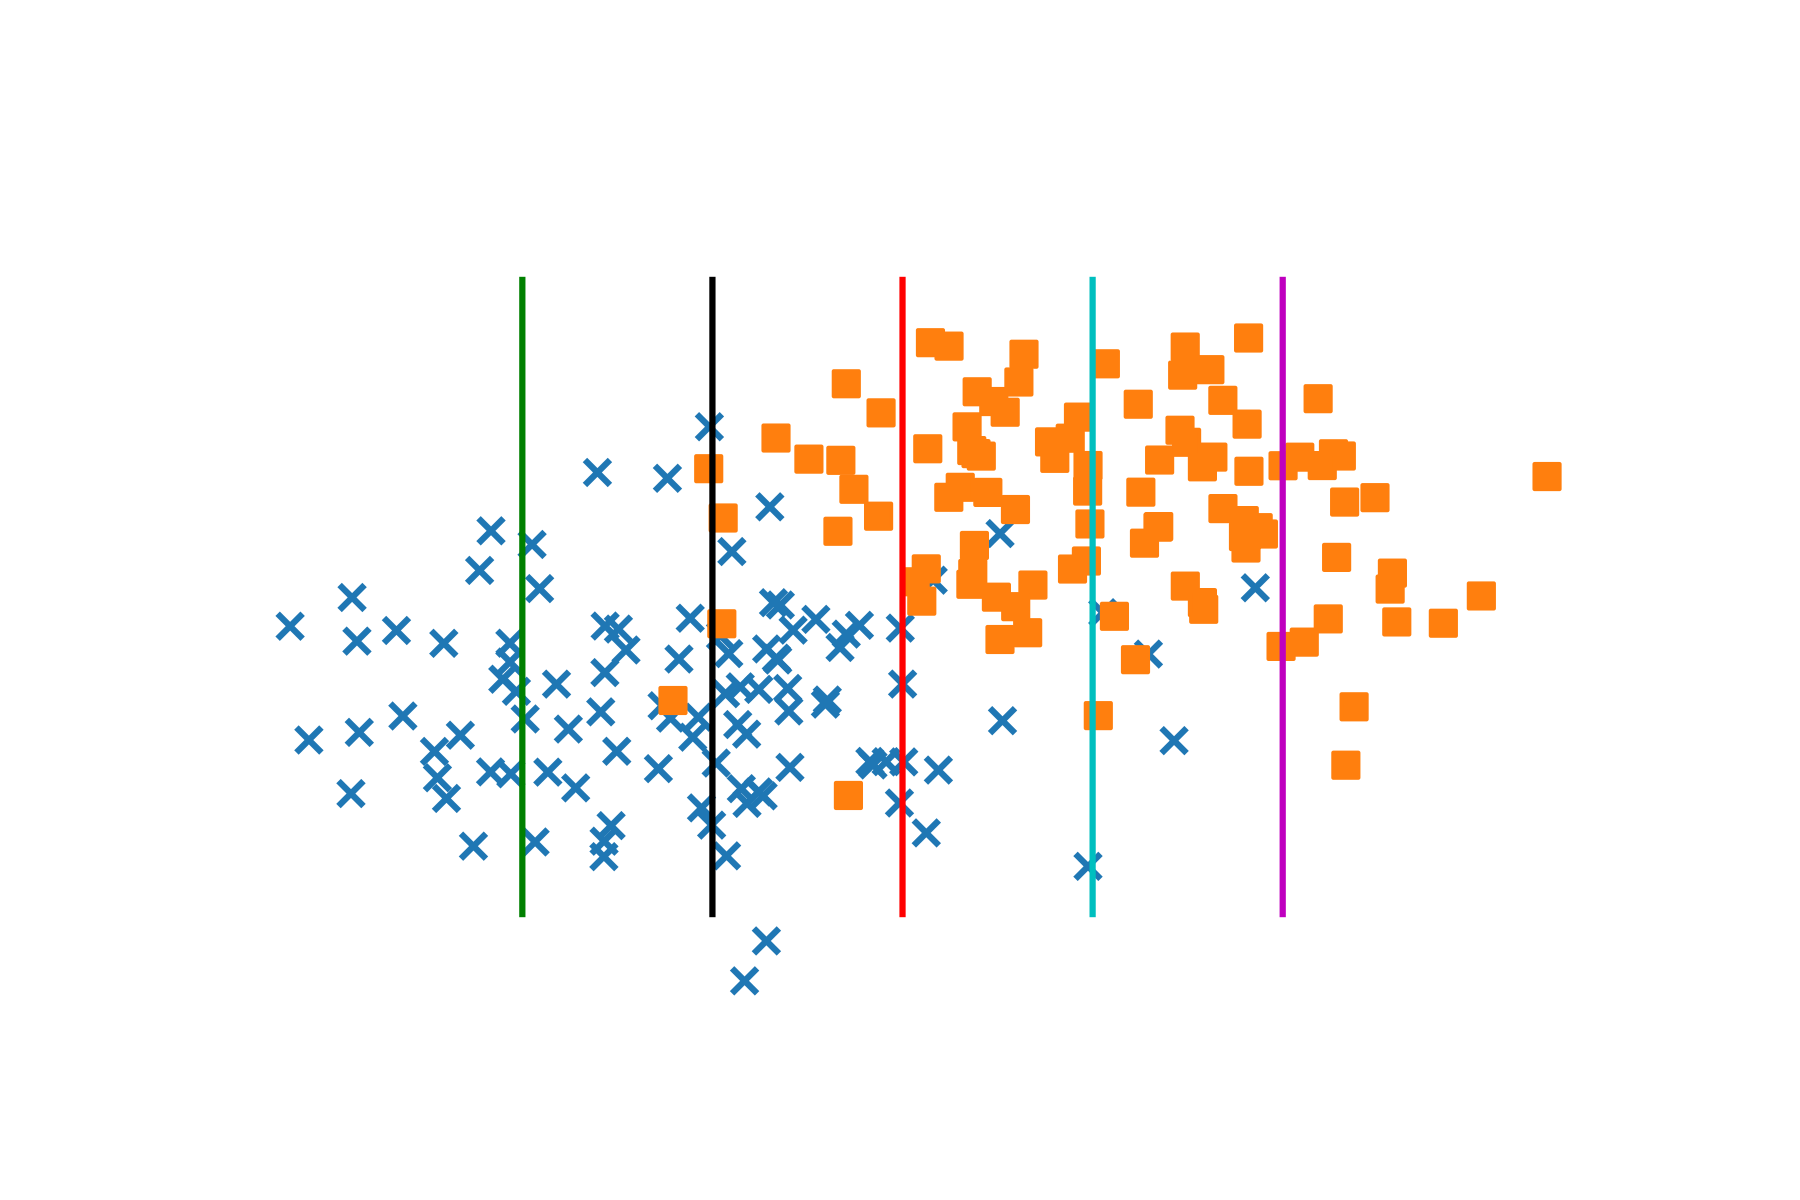
\includegraphics[width=1.\textwidth]{split.png}
		\end{figure}
	\end{column}
\end{columns}

\begin{textblock*}{.1\paperheight}(0.28\paperwidth, 0.71\paperheight)
	\only<2>{
\includegraphics[width=1.\textwidth]{Axe}}
\end{textblock*}

\end{frame}

%------------------------------------------------

\begin{frame}

\myframetitle{0.27\paperwidth}{0.04\paperwidth}{\insertsection}
\myframesubtitle{0.29\paperwidth}{\insertsubsection}

\vspace{0.2\paperheight}
\begin{itemize}
	%			\itemsep0.8ex
	\small
	\setbeamertemplate{items}{\mybullet}
	\item Suppose we have n features $x^{(1)}, x^{(2)}, ..., x^{(n)}$ in our dataset X

	\item If we want to split on some feature $x^{(j)}$ at threshold $t$ then we propose\\ to maximize \textbf{Information Gain} (IG):
\[
\text{IG}(\text{X}, \text{a})=\mathrm{H}(\text{X})-\mathrm{H}(\text{X} \mid \text{a}) \rightarrow \max_\text{a}
\]
\[ 
\mathrm{H}(\text{X} \mid \text{a})=\sum_{v \in v a l s(\text{a})} \frac{\left|S_{\text{a}}(v)\right|}{|\text{X}|} \cdot \mathrm{H}\left(S_{\text{a}}(v)\right)
\]

\item In case of a binary tree with L(R) elements in the left (right) split we've got: 
\[
\text{H}(X, j, t) = 
\dfrac{|\text{L}|}{|\text{X}|}\mathrm{H}(\text{L}) + \dfrac{|\text{R}|}{|\text{X}|}\mathrm{H}(\text{R}) \rightarrow \min_{j, t}
\]
%\[
%IG(j, t) = 
%\dfrac{|L|}{|X|}H(L) + \dfrac{|R|}{|X|}H(R) \rightarrow \min_{j, t}
%\]
\vfill
\onslide<2>{\centering \textcolor{myorange}{How to choose H(X)?}}
%\textcolor{mypurple}{Look on the best split}}

\end{itemize}
% \onslide<2>{\begin{tikzpicture}[remember picture,overlay]
%     \node [shift={(1.0em,-4.0ex)}, anchor=west] at ({pic cs:start1a}) (X) {H(X)?};
%     \draw [red, thick, -latex] (X.west) -| ($({pic cs:start1a})!0.5!({pic cs:end1a})+(0,-0.5ex)$);
%     \draw [red, thick, -latex] (X.east) -| ($({pic cs:start2a})!0.5!({pic cs:end2a})+(0,-0.5ex)$);
% \end{tikzpicture}}

\begin{textblock*}{0.45\paperwidth}(0.8\paperwidth,0.1\paperheight)
	\footnotesize
	\textcolor{Gray}{\href{https://en.wikipedia.org/wiki/Information_gain_in_decision_trees}{\underline{more about IG}} }
\end{textblock*}

\end{frame}

%------------------------------------------------

\begin{frame}
\myframetitle{0.27\paperwidth}{0.04\paperwidth}{\insertsection}
\myframesubtitle{0.29\paperwidth}{\insertsubsection}

\vspace{0.1\paperheight}
\begin{columns}
\begin{column}{0.5\textwidth}
\begin{figure}
	\centering
	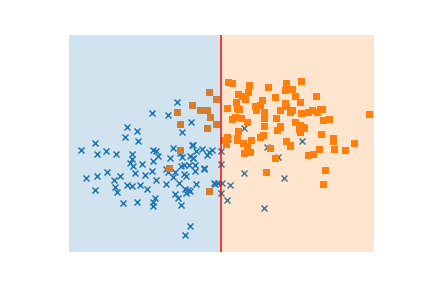
\includegraphics[width=1.\textwidth]{psplit.png}
\end{figure}
\end{column}

\begin{column}{0.5\textwidth}
\begin{figure}
	
\includegraphics[width=.3\textwidth]{Axe.png}
\end{figure}
\end{column}
\end{columns}

\vfill
The "best" split is a central one because it introduces \textbf{purity} in the best way. And we have some functions to measure the purity!
\end{frame}

%------------------------------------------------

\begin{frame}
\myframetitle{0.27\paperwidth}{0.04\paperwidth}{\insertsection}
\myframesubtitle{0.29\paperwidth}{\insertsubsection}

\centering
\vspace{1.5cm}
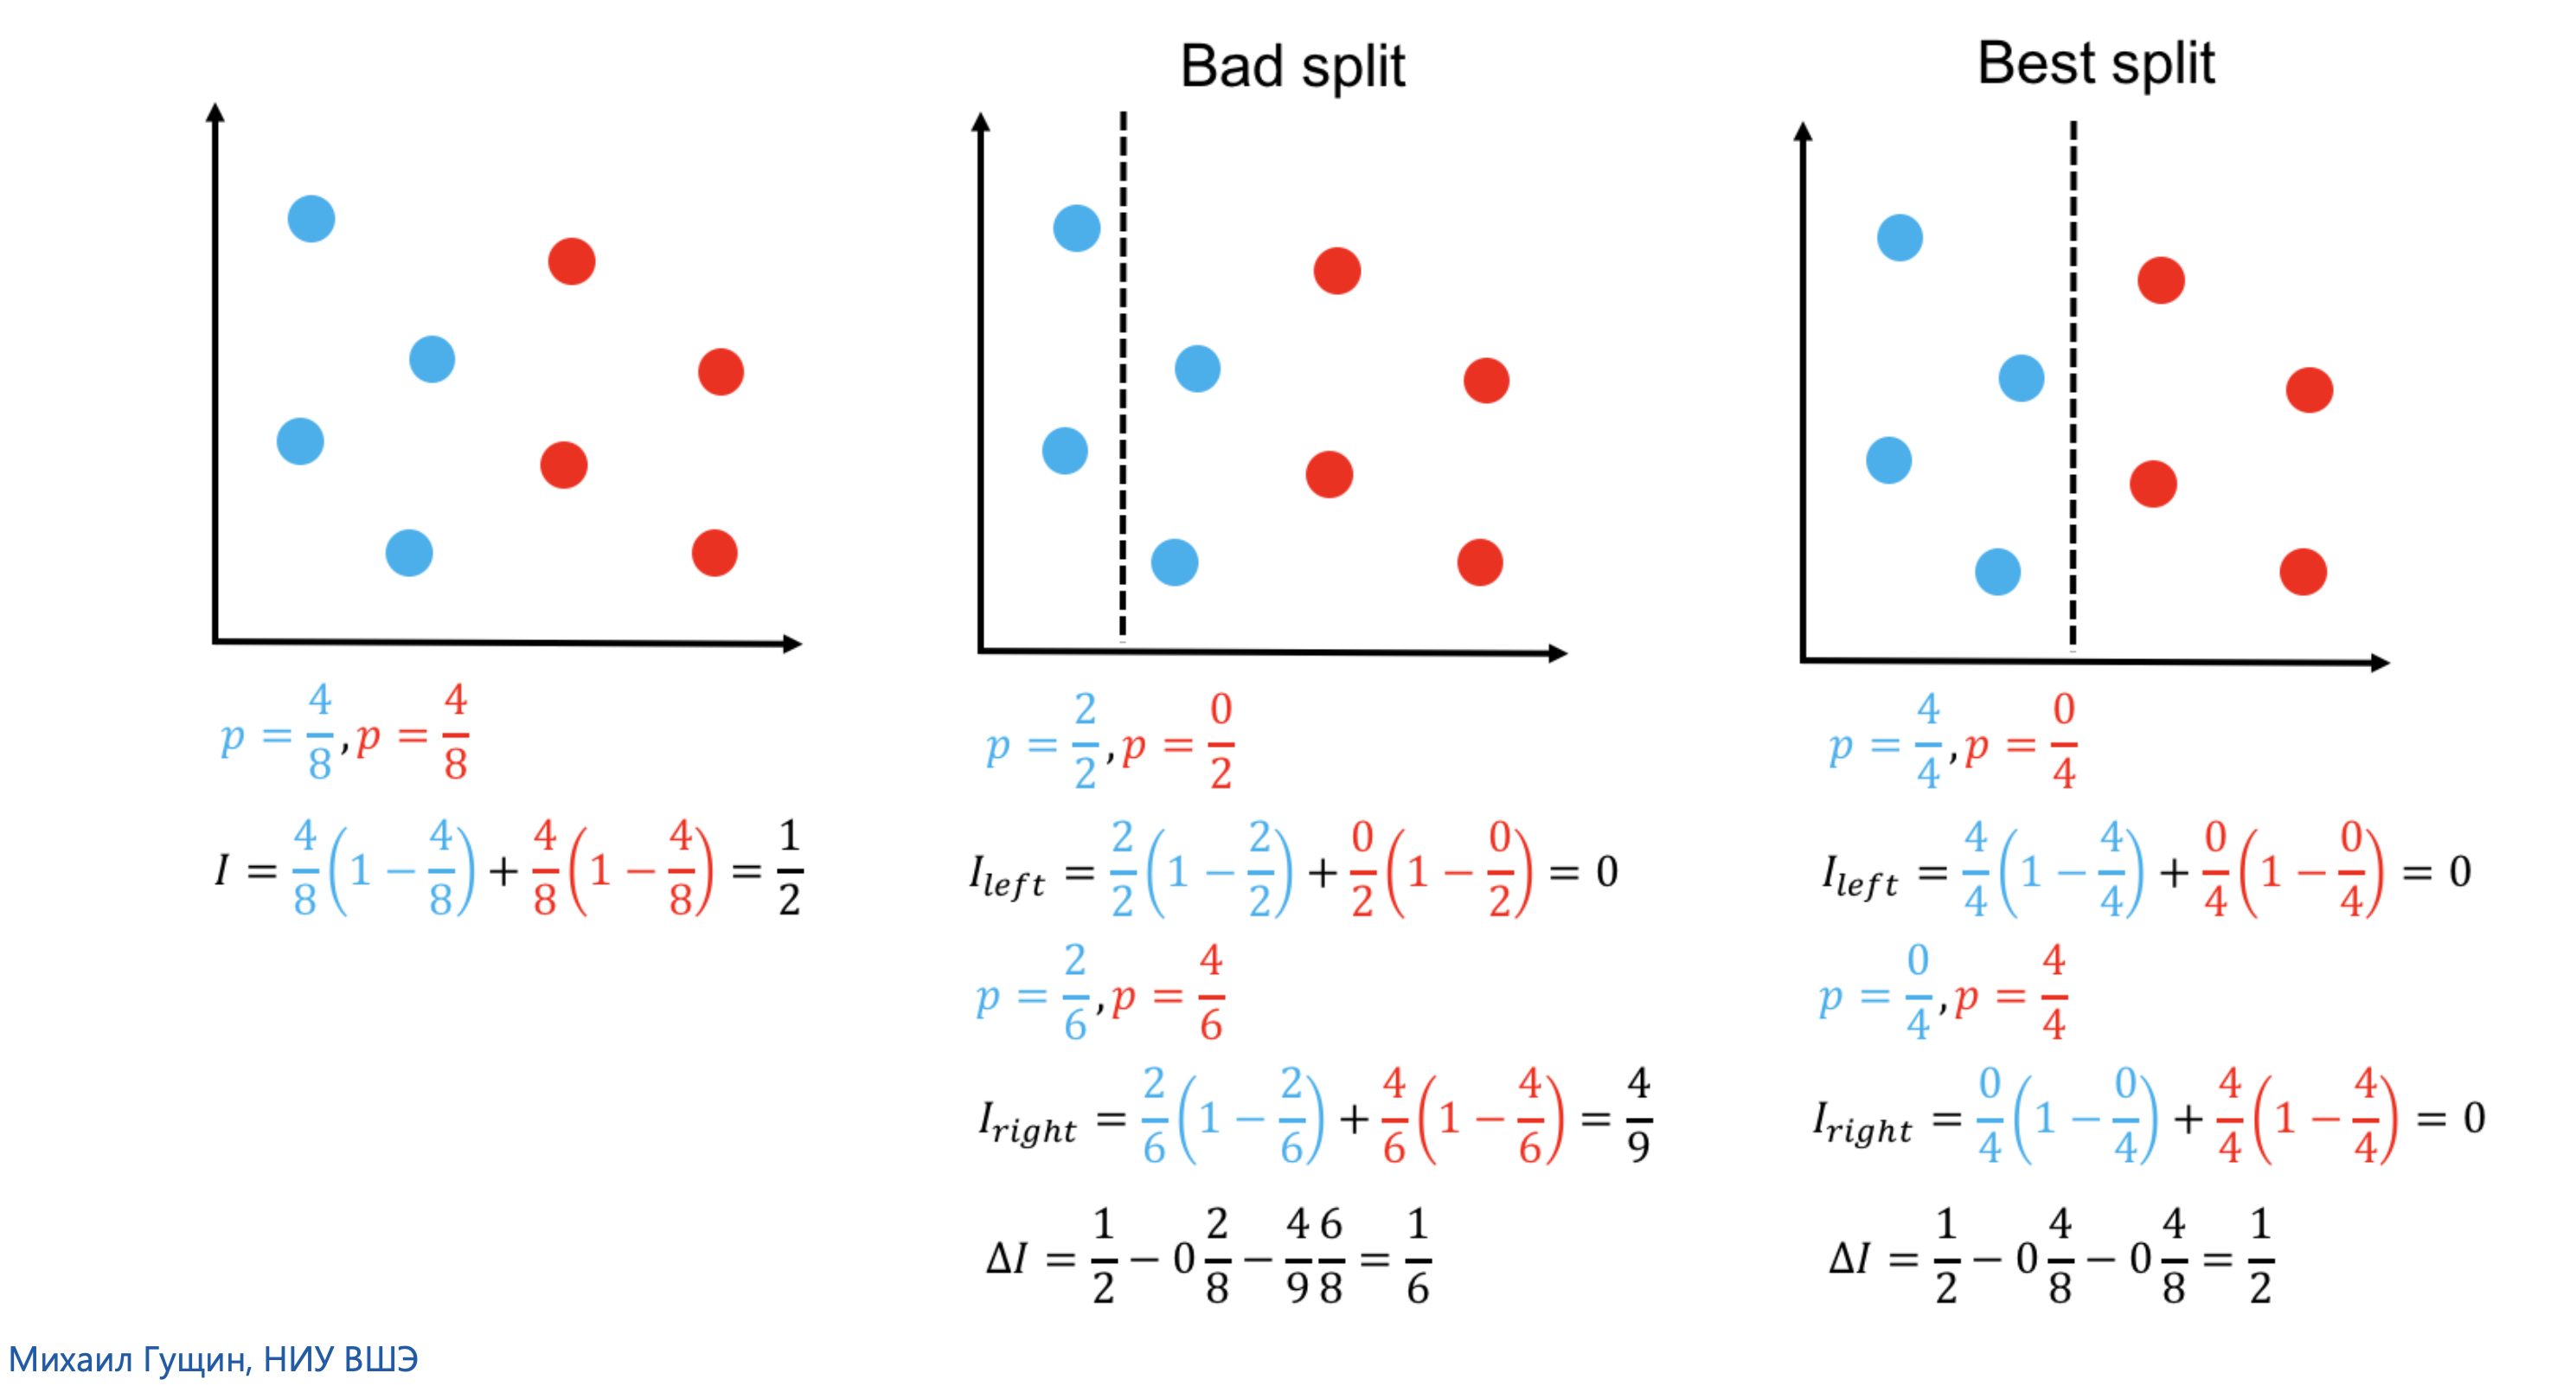
\includegraphics[width=0.9\linewidth]{gini_criterion.png}

\end{frame}

%------------------------------------------------

\begin{frame}
\myframetitle{0.27\paperwidth}{0.04\paperwidth}{\insertsection}
\myframesubtitle{0.29\paperwidth}{\insertsubsection}

\centering
\vspace{1.5cm}
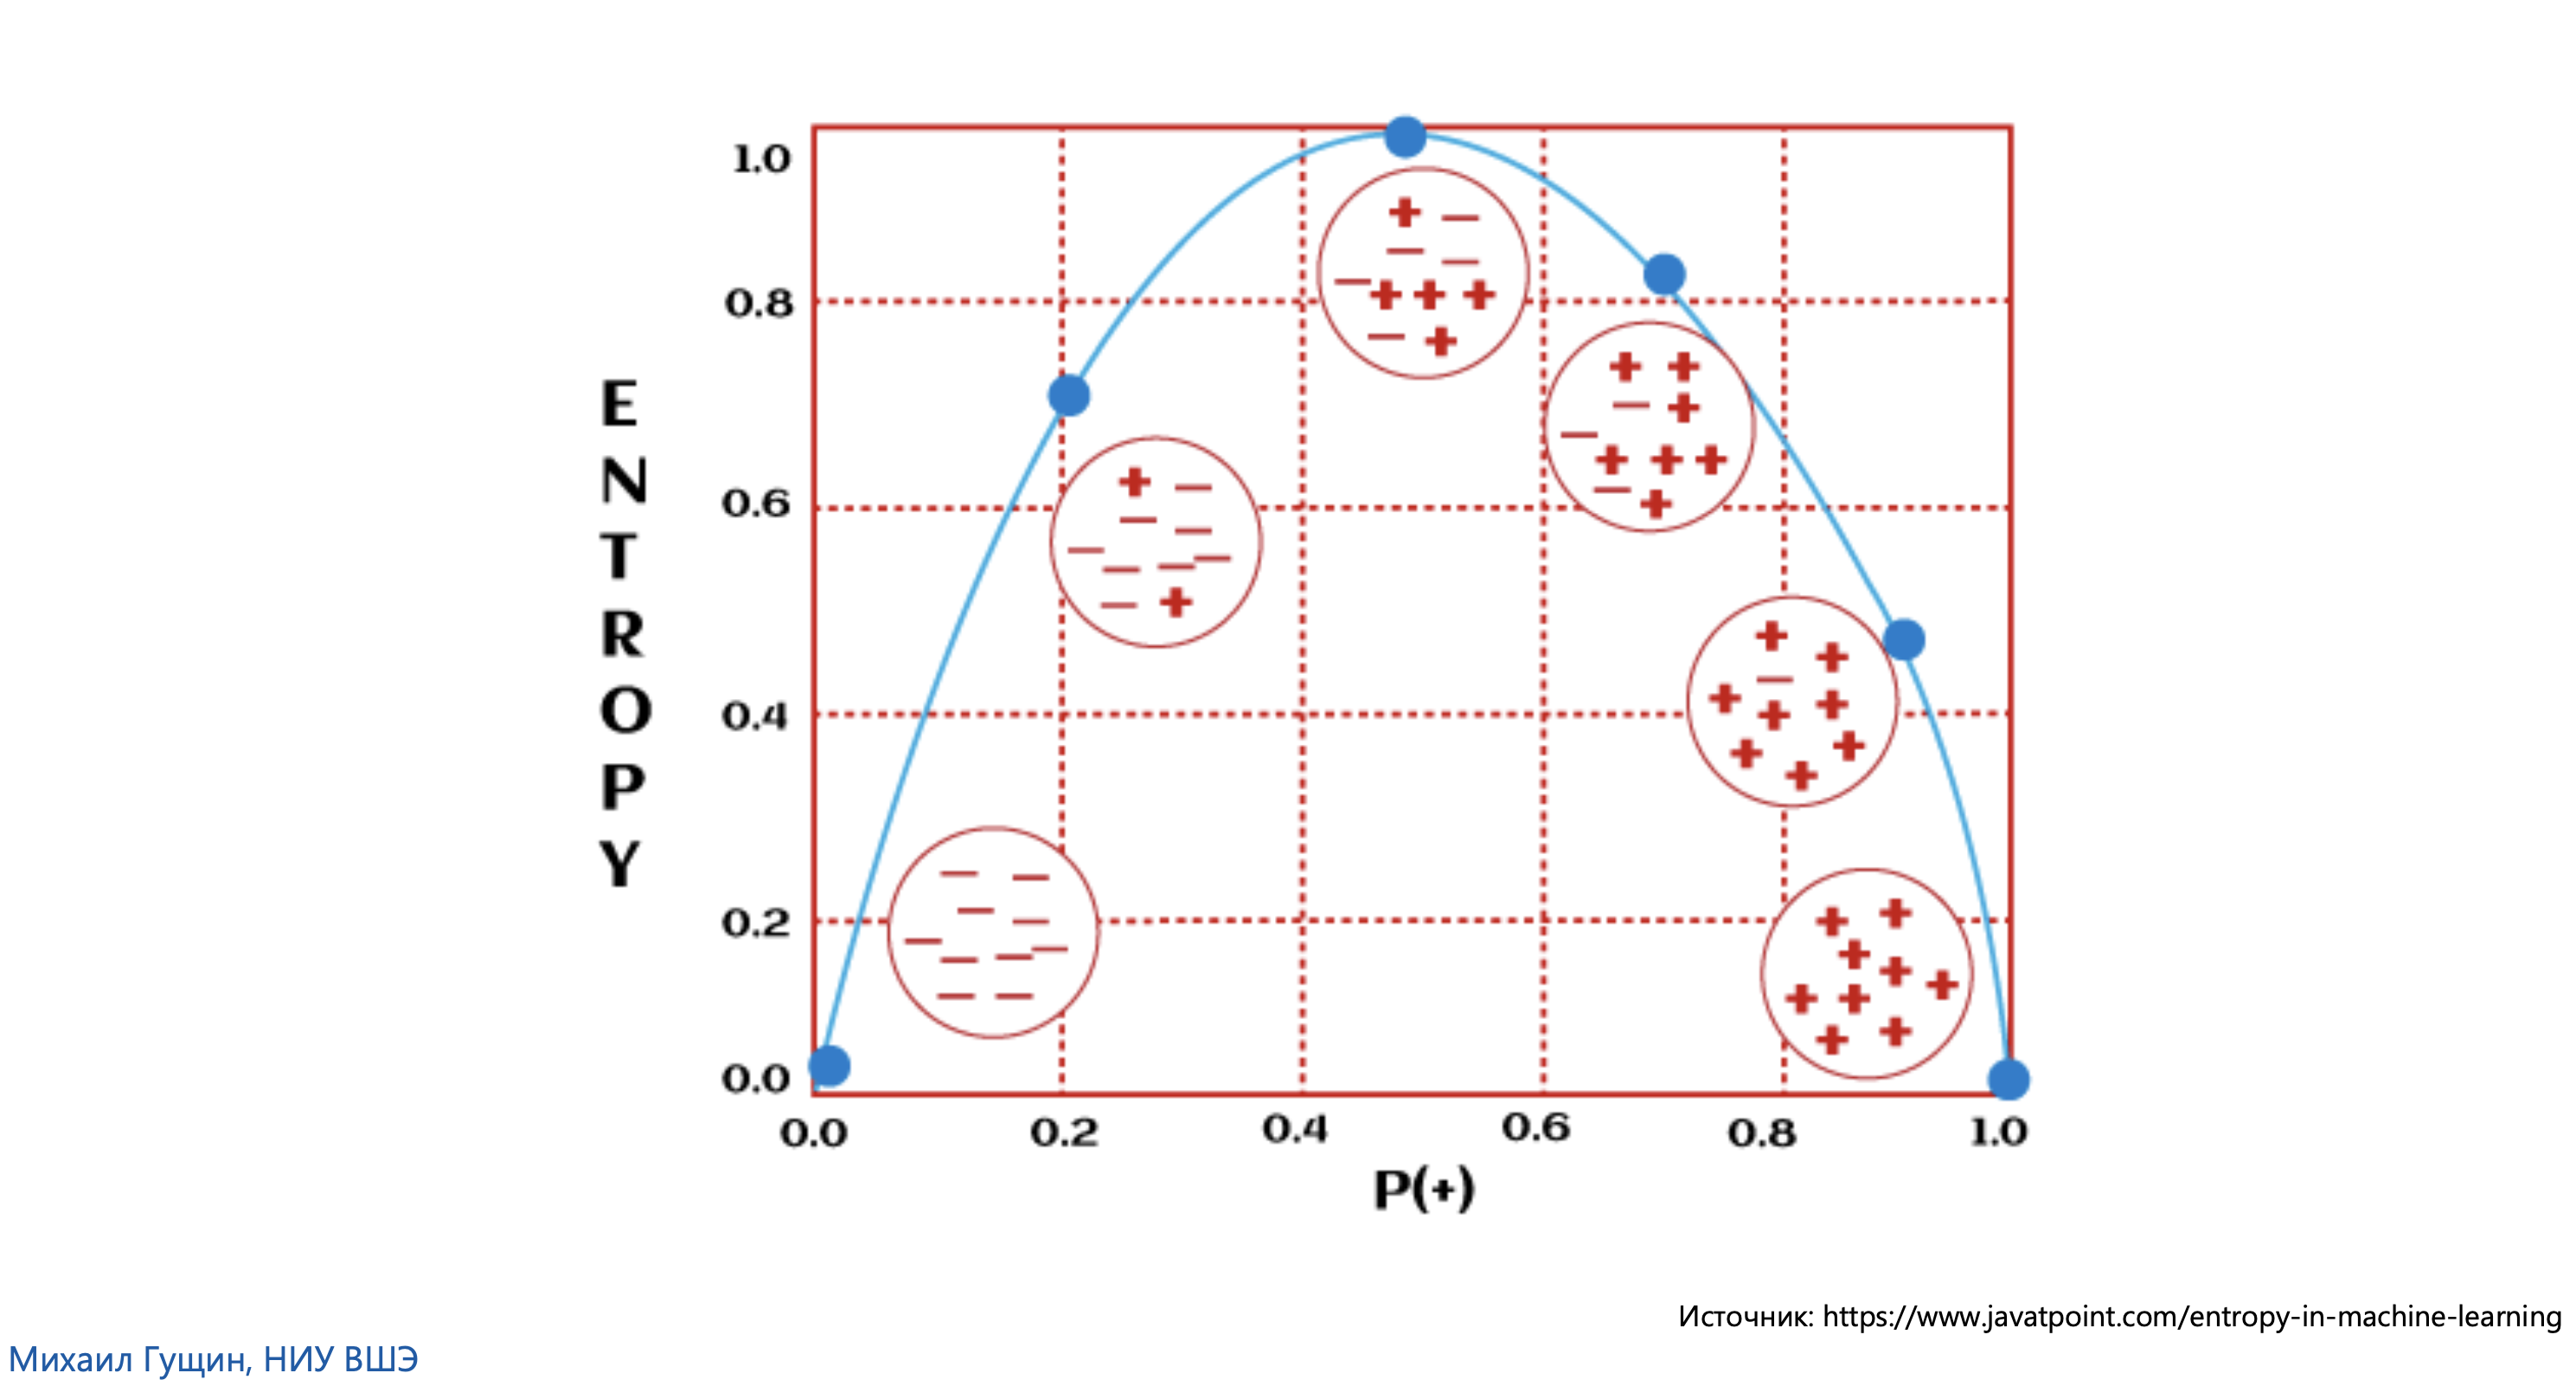
\includegraphics[width=0.9\linewidth]{entropy_criterion.png}

\end{frame}

%------------------------------------------------

\begin{frame}
\myframetitle{0.27\paperwidth}{0.04\paperwidth}{\insertsection}
\myframesubtitle{0.29\paperwidth}{\insertsubsection}

\centering
\vspace{1.5cm}
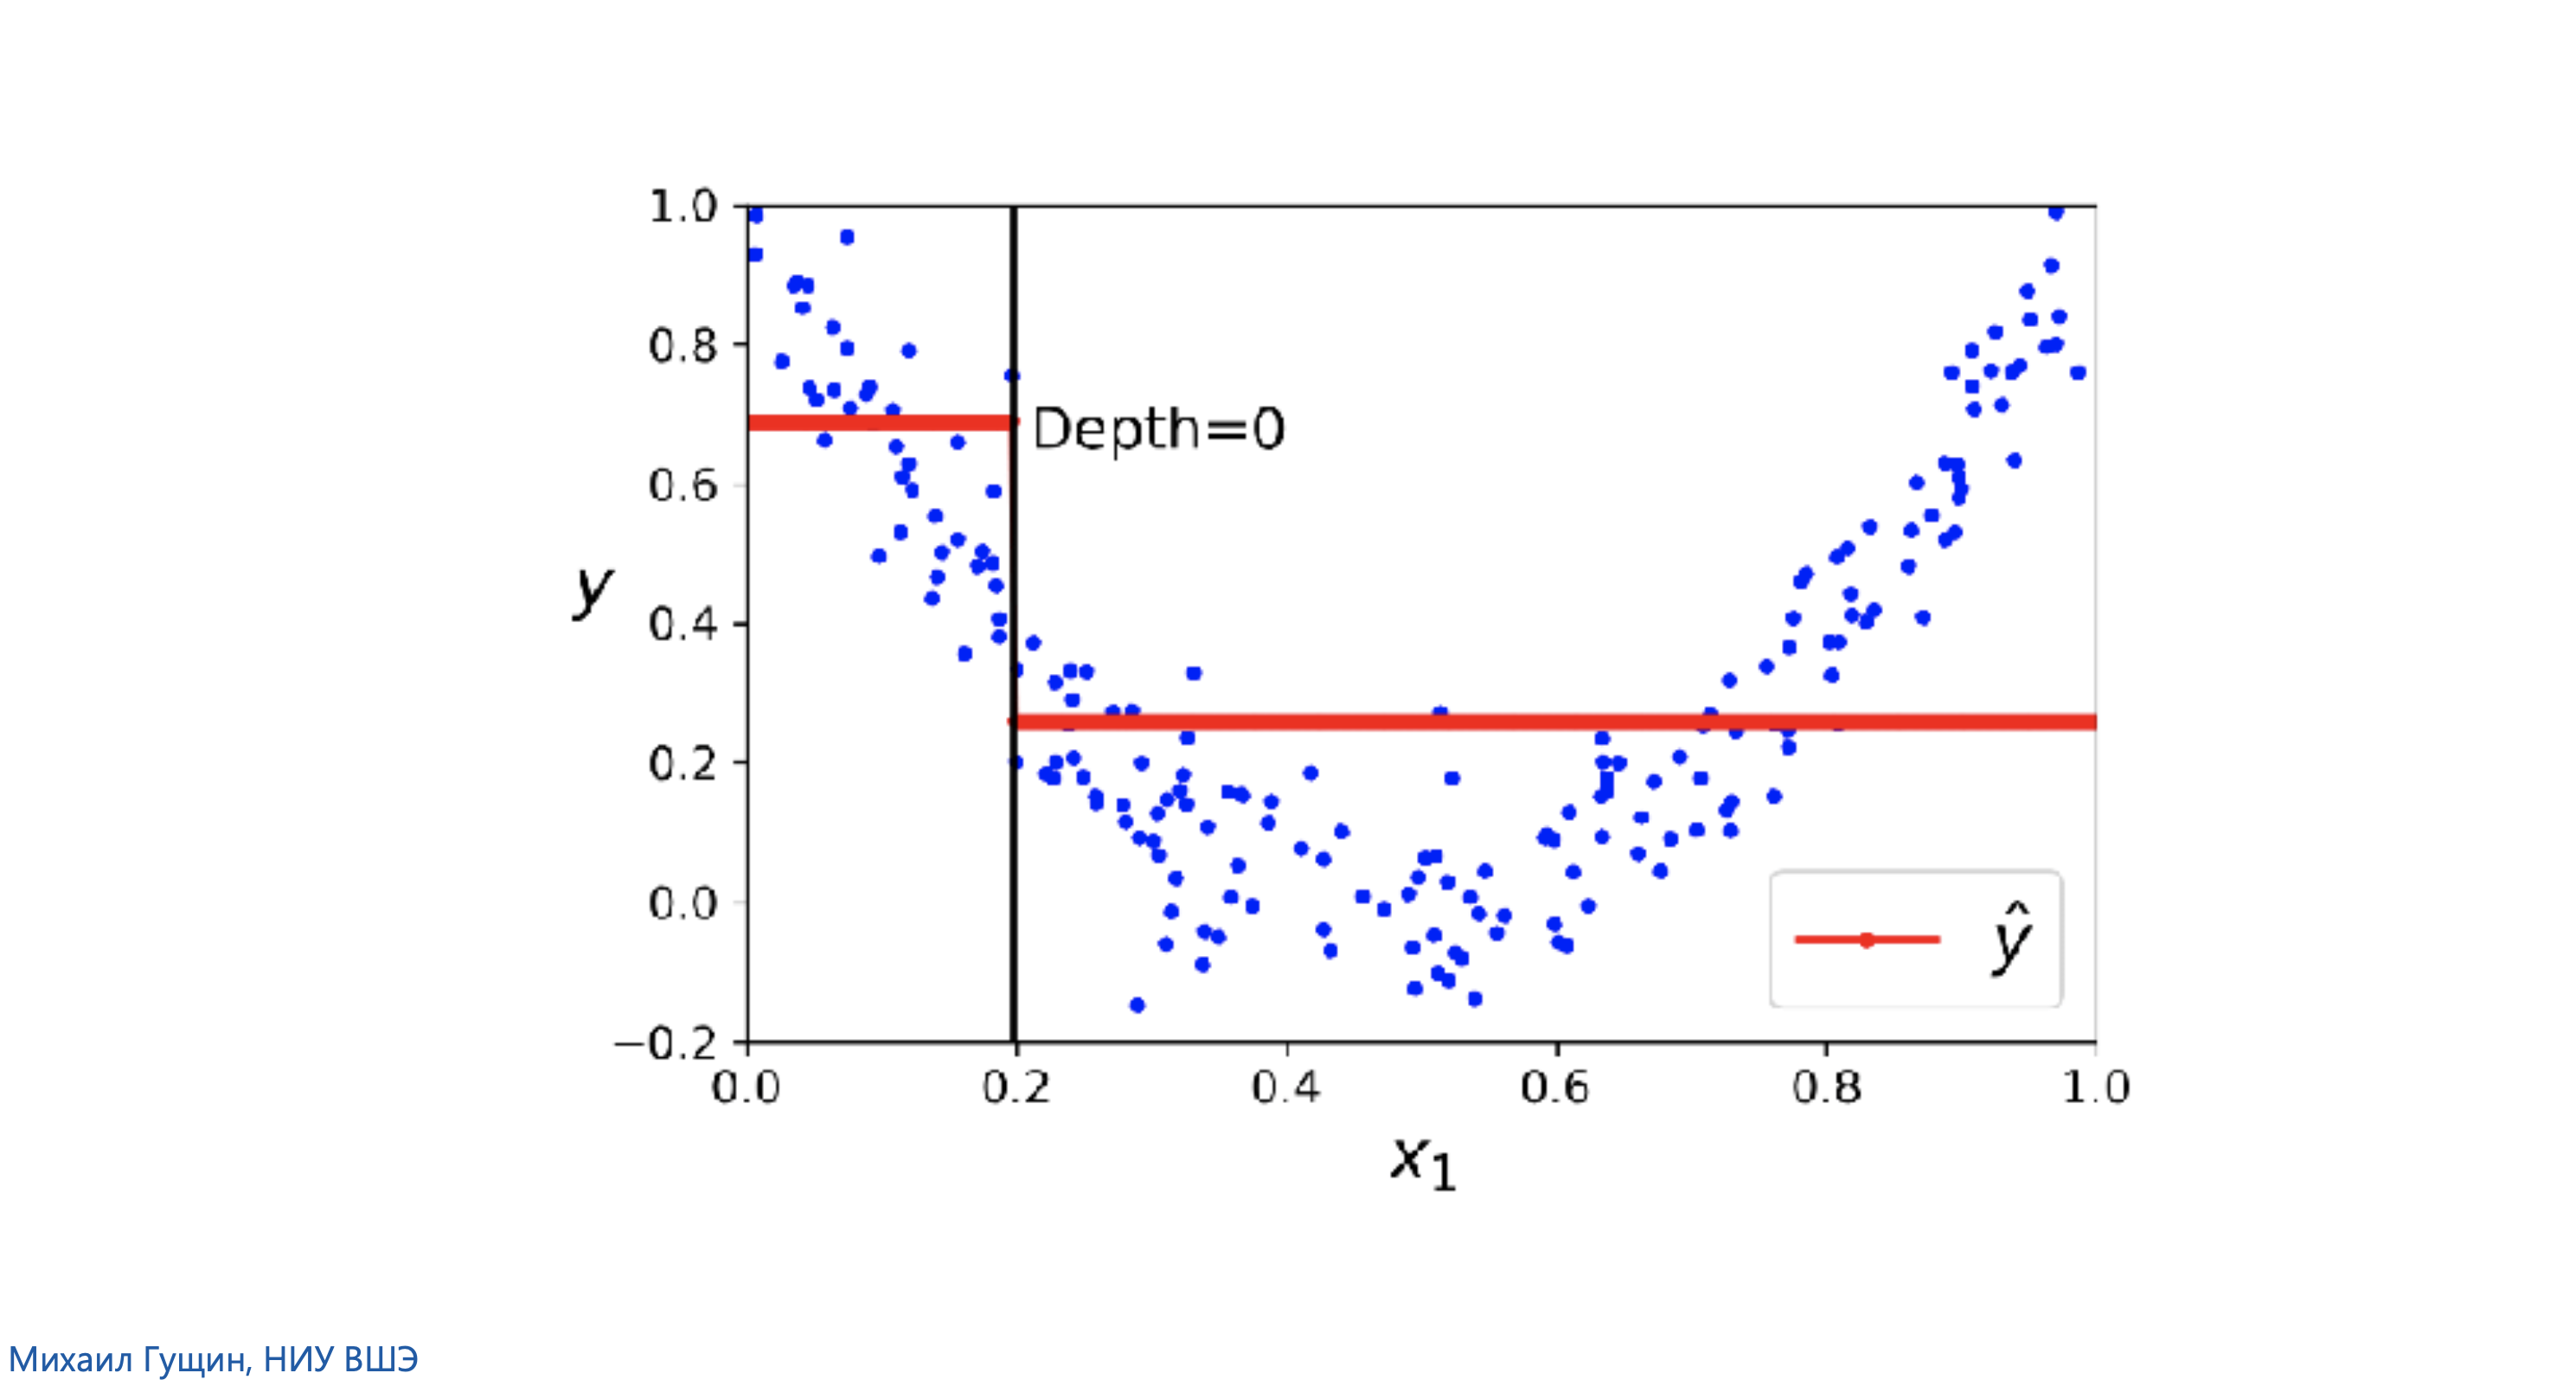
\includegraphics[width=0.9\linewidth]{regression_criterion.png}

\end{frame}
%------------------------------------------------

\subsection{regression}
\begin{frame}
\myframetitle{0.27\paperwidth}{0.04\paperwidth}{\insertsection}
\myframesubtitle{0.29\paperwidth}{\insertsubsection}

\vspace{0.1\paperheight}
\begin{figure}
\centering
\only<1>{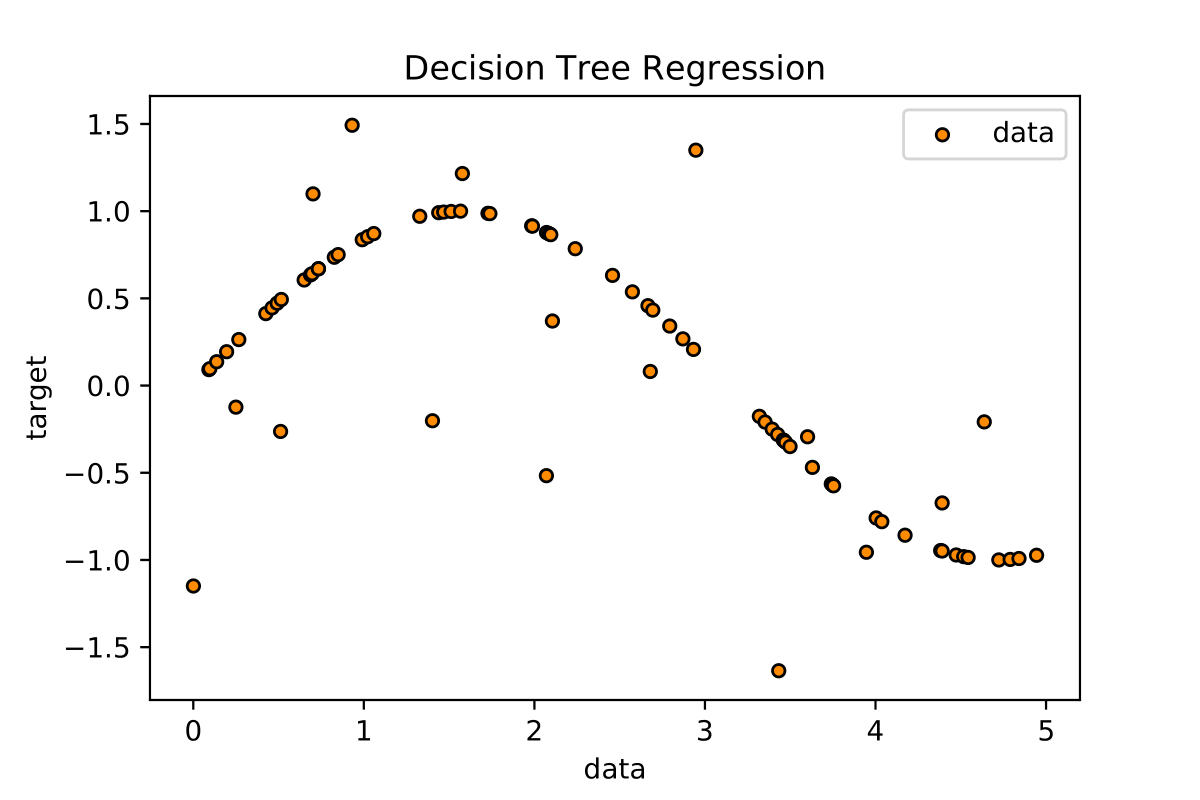
\includegraphics[width=0.6\textwidth]{regression.png}}
\only<2>{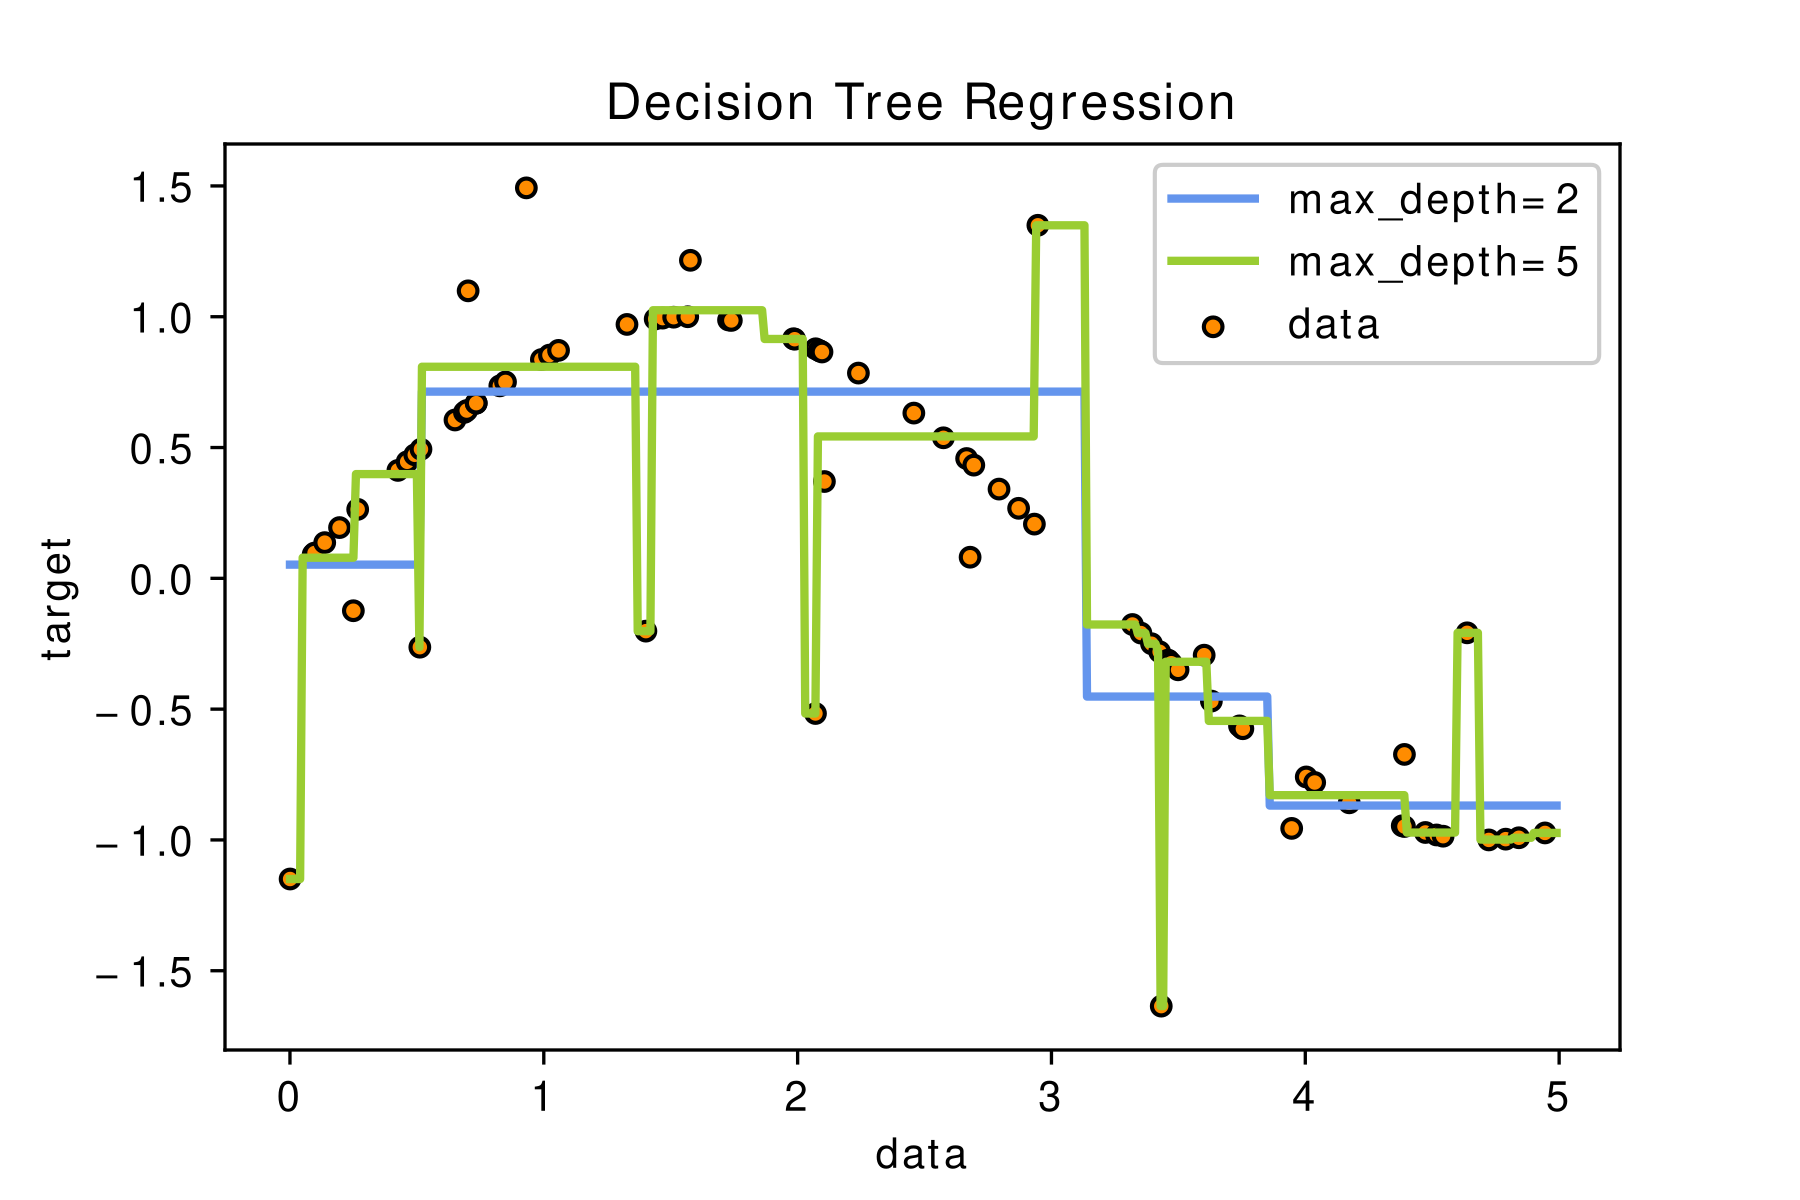
\includegraphics[width=0.6\textwidth]{dregr.png}}
\end{figure}
\centering
\small
Can we use decision tree approach for regression problem?
\only<2>{\textcolor{myorange}{Yes}}
\end{frame}

%------------------------------------------------

\subsection{growing}
\begin{frame}
\myframetitle{0.27\paperwidth}{0.04\paperwidth}{\insertsection}
\myframesubtitle{0.29\paperwidth}{\insertsubsection}

\vspace{-0.15\paperheight}
What about tree construction? \onslide<2->{\textcolor{myorange}{Do it recursively by \textbf{greedy} algorithm}}

\begin{textblock*}{1\paperwidth}(0.02\paperwidth, 0.35\paperheight)
	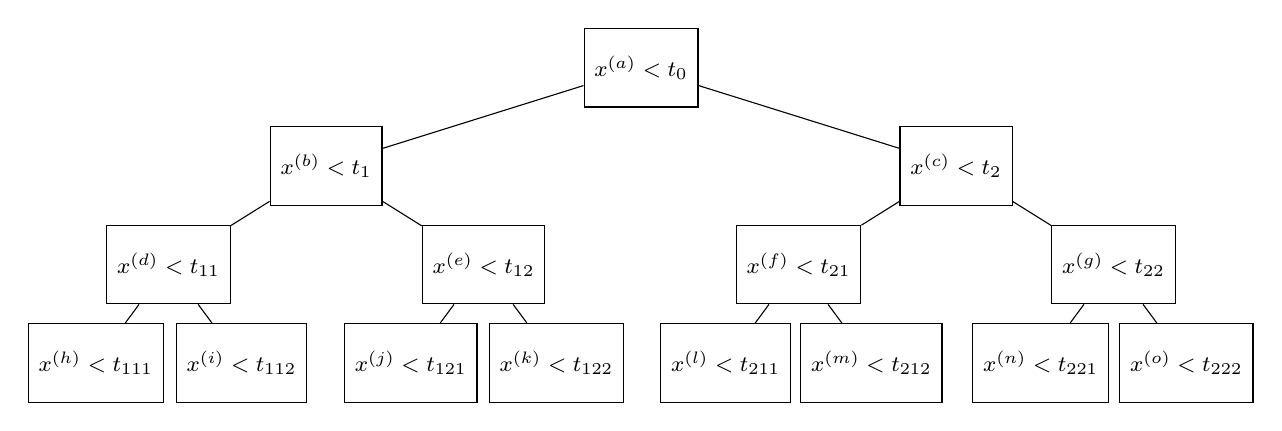
\begin{tikzpicture}[scale=0.5]
	\footnotesize	
	\node [arn_n] {$x^{(a)} < t_0$}
	child[visible on=<2->]{ node [arn_n] {$x^{(b)} < t_1$}
		child[visible on=<3->]{ node [arn_n] {$x^{(d)} < t_{11}$}
			child[visible on=<4->]{ node [arn_n] {$x^{(h)} < t_{111}$}}
			child[visible on=<4->]{ node [arn_n] {$x^{(i)} < t_{112}$}}                          
		}
		child[visible on=<3->]{ node [arn_n] {$x^{(e)} < t_{12}$}  
			child[visible on=<4->]{ node [arn_n] {$x^{(j)} < t_{121}$}}
			child[visible on=<4->]{ node [arn_n] {$x^{(k)} < t_{122}$}}                          
		}
	}
	child[visible on=<2->]{ node [arn_n] {$x^{(c)} < t_2$}
		child[visible on=<3->]{ node [arn_n] {$x^{(f)} < t_{21}$}
			child[visible on=<4->]{ node [arn_n] {$x^{(l)} < t_{211}$}}
			child[visible on=<4->]{ node [arn_n] {$x^{(m)} < t_{212}$}}                          
		}
		child[visible on=<3->]{ node [arn_n] {$x^{(g)} < t_{22}$}  
			child[visible on=<4->]{ node [arn_n] {$x^{(n)} < t_{221}$}}
			child[visible on=<4->]{ node [arn_n] {$x^{(o)} < t_{222}$}}                          
		}
	}
	%	}
	%}
	; 
	\end{tikzpicture} 
\end{textblock*}

\end{frame}

%------------------------------------------------

%\subsection{examples}
\begin{frame}
\myframetitle{0.27\paperwidth}{0.04\paperwidth}{\insertsection}
\myframesubtitle{0.29\paperwidth}{\insertsubsection}

\vspace{0.05\paperheight}
\begin{columns}
\begin{column}{0.5\textwidth}
	
	\only<1>{
		\begin{figure}
			\centering
			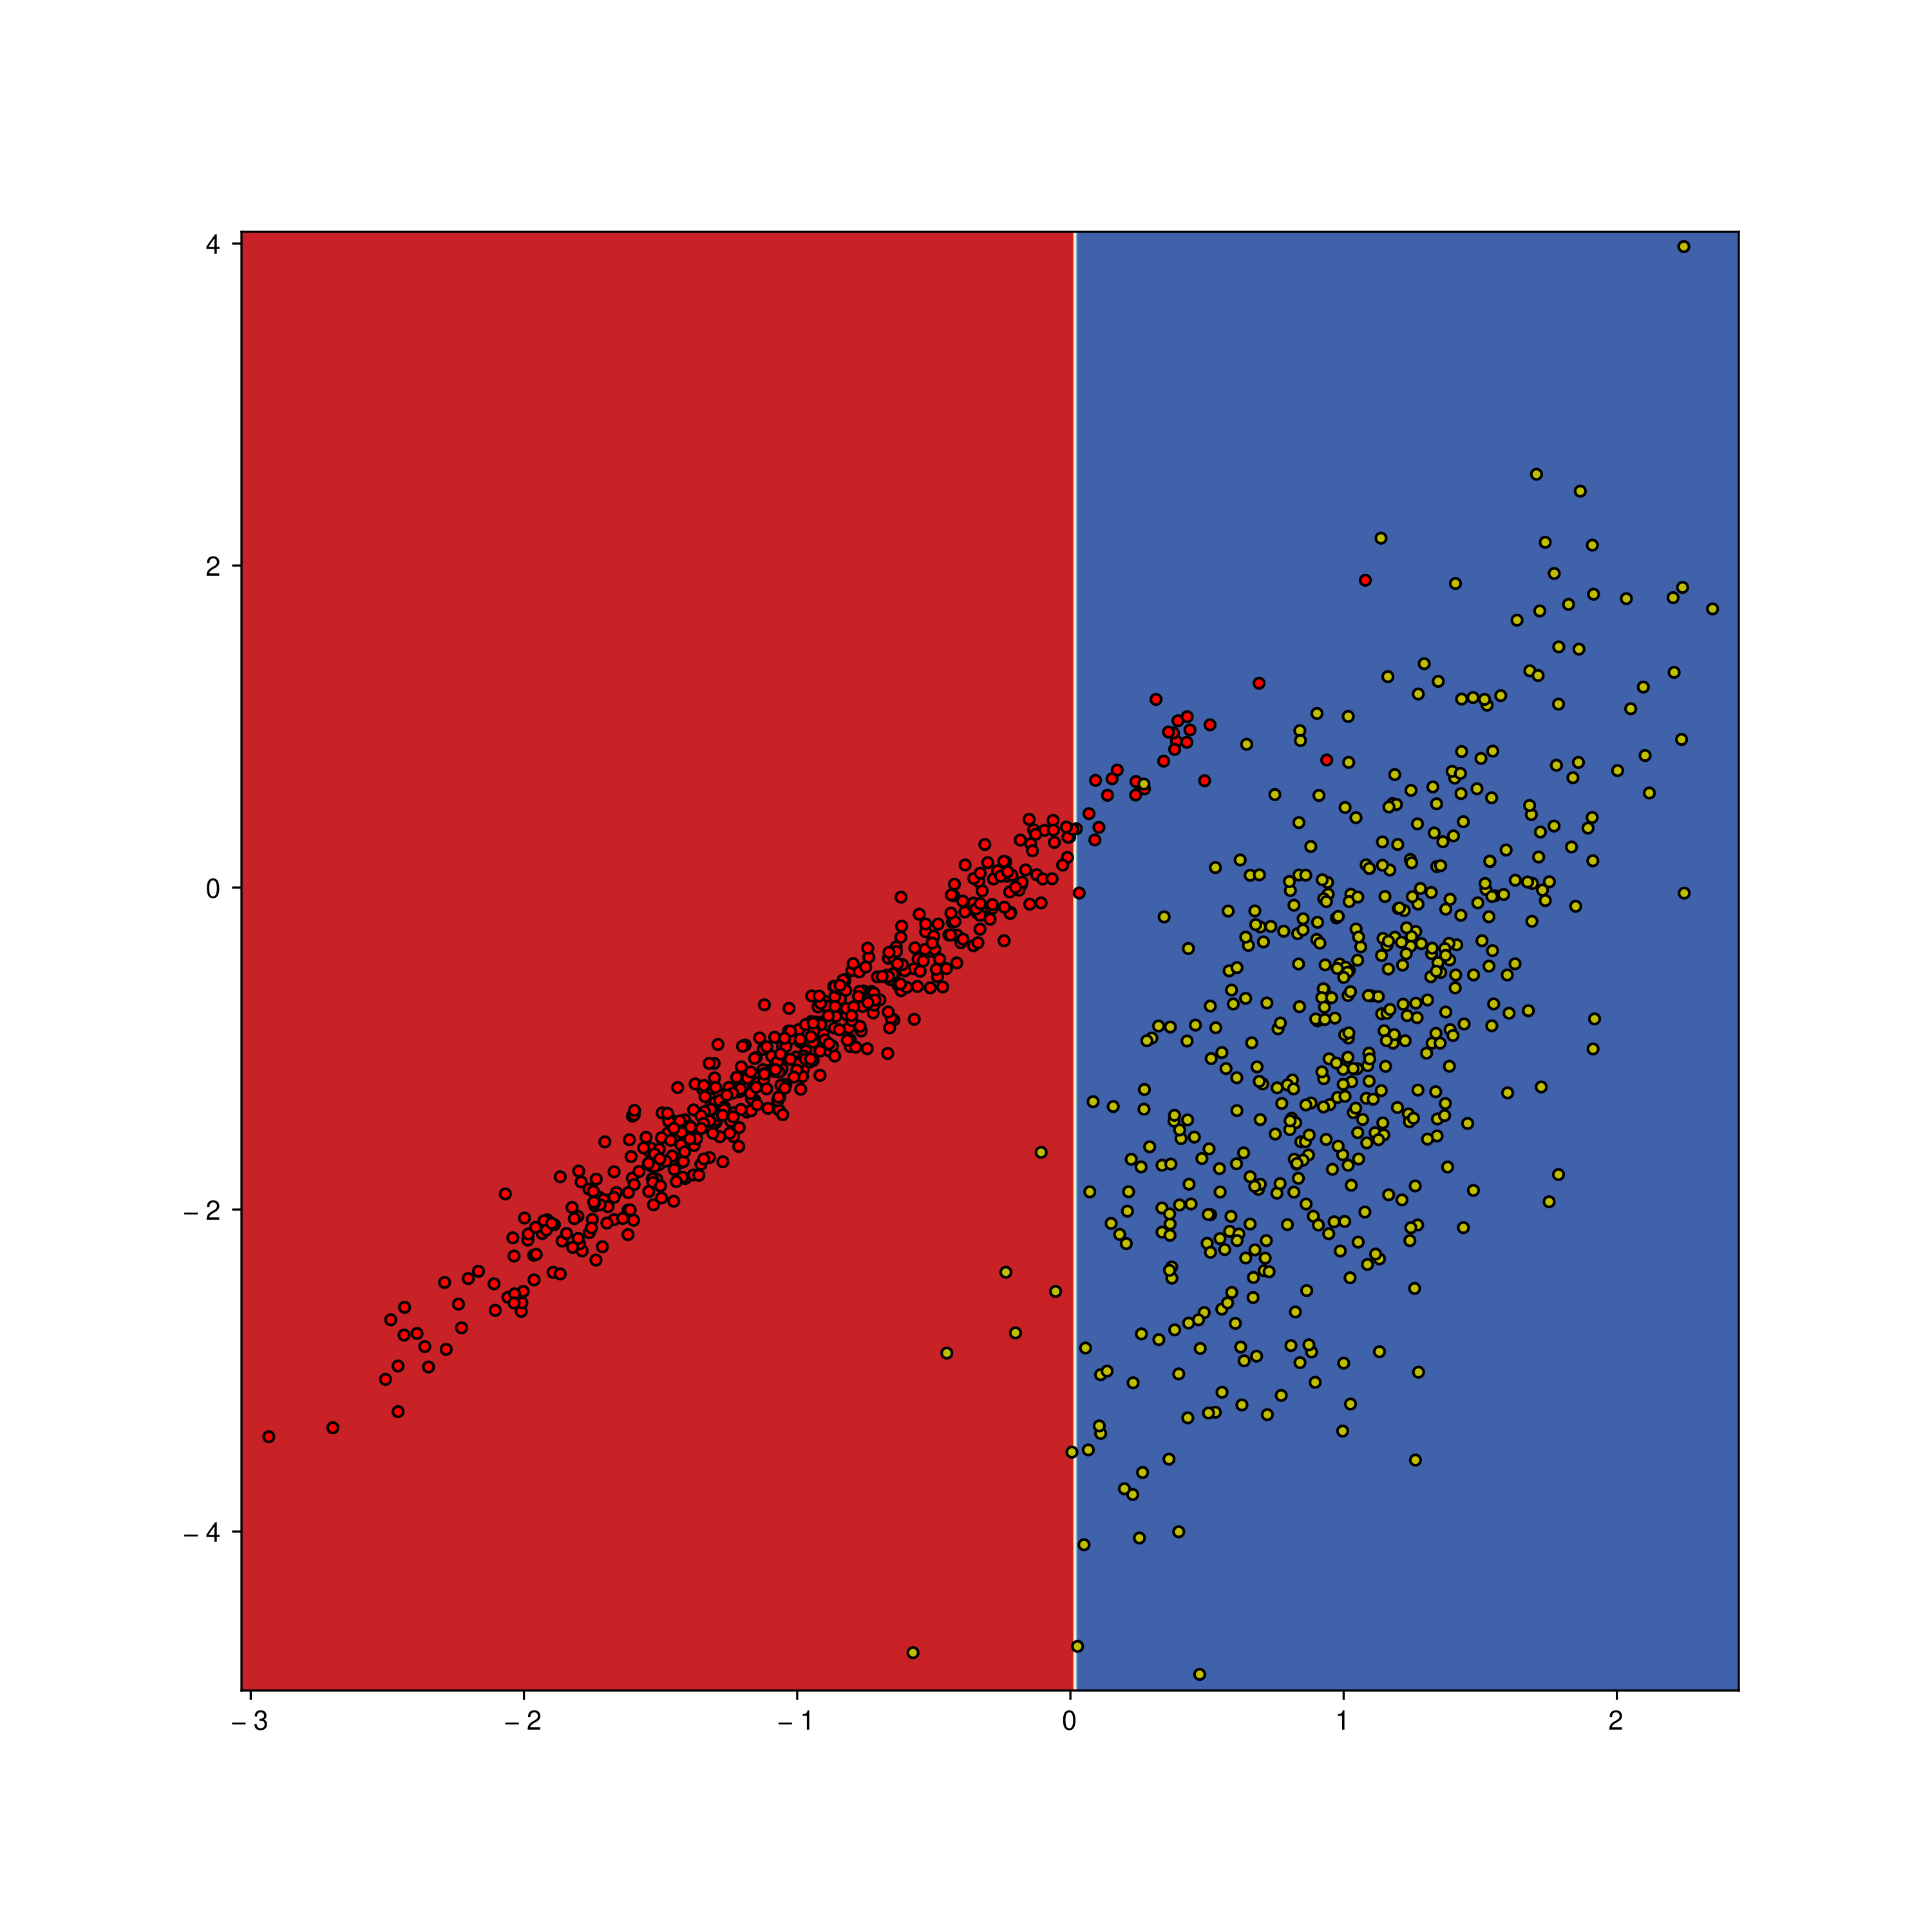
\includegraphics[width=0.7\textheight]{1gi.png}
		\end{figure}
	}
	
	\only<2>{
		\begin{figure}
			\centering
			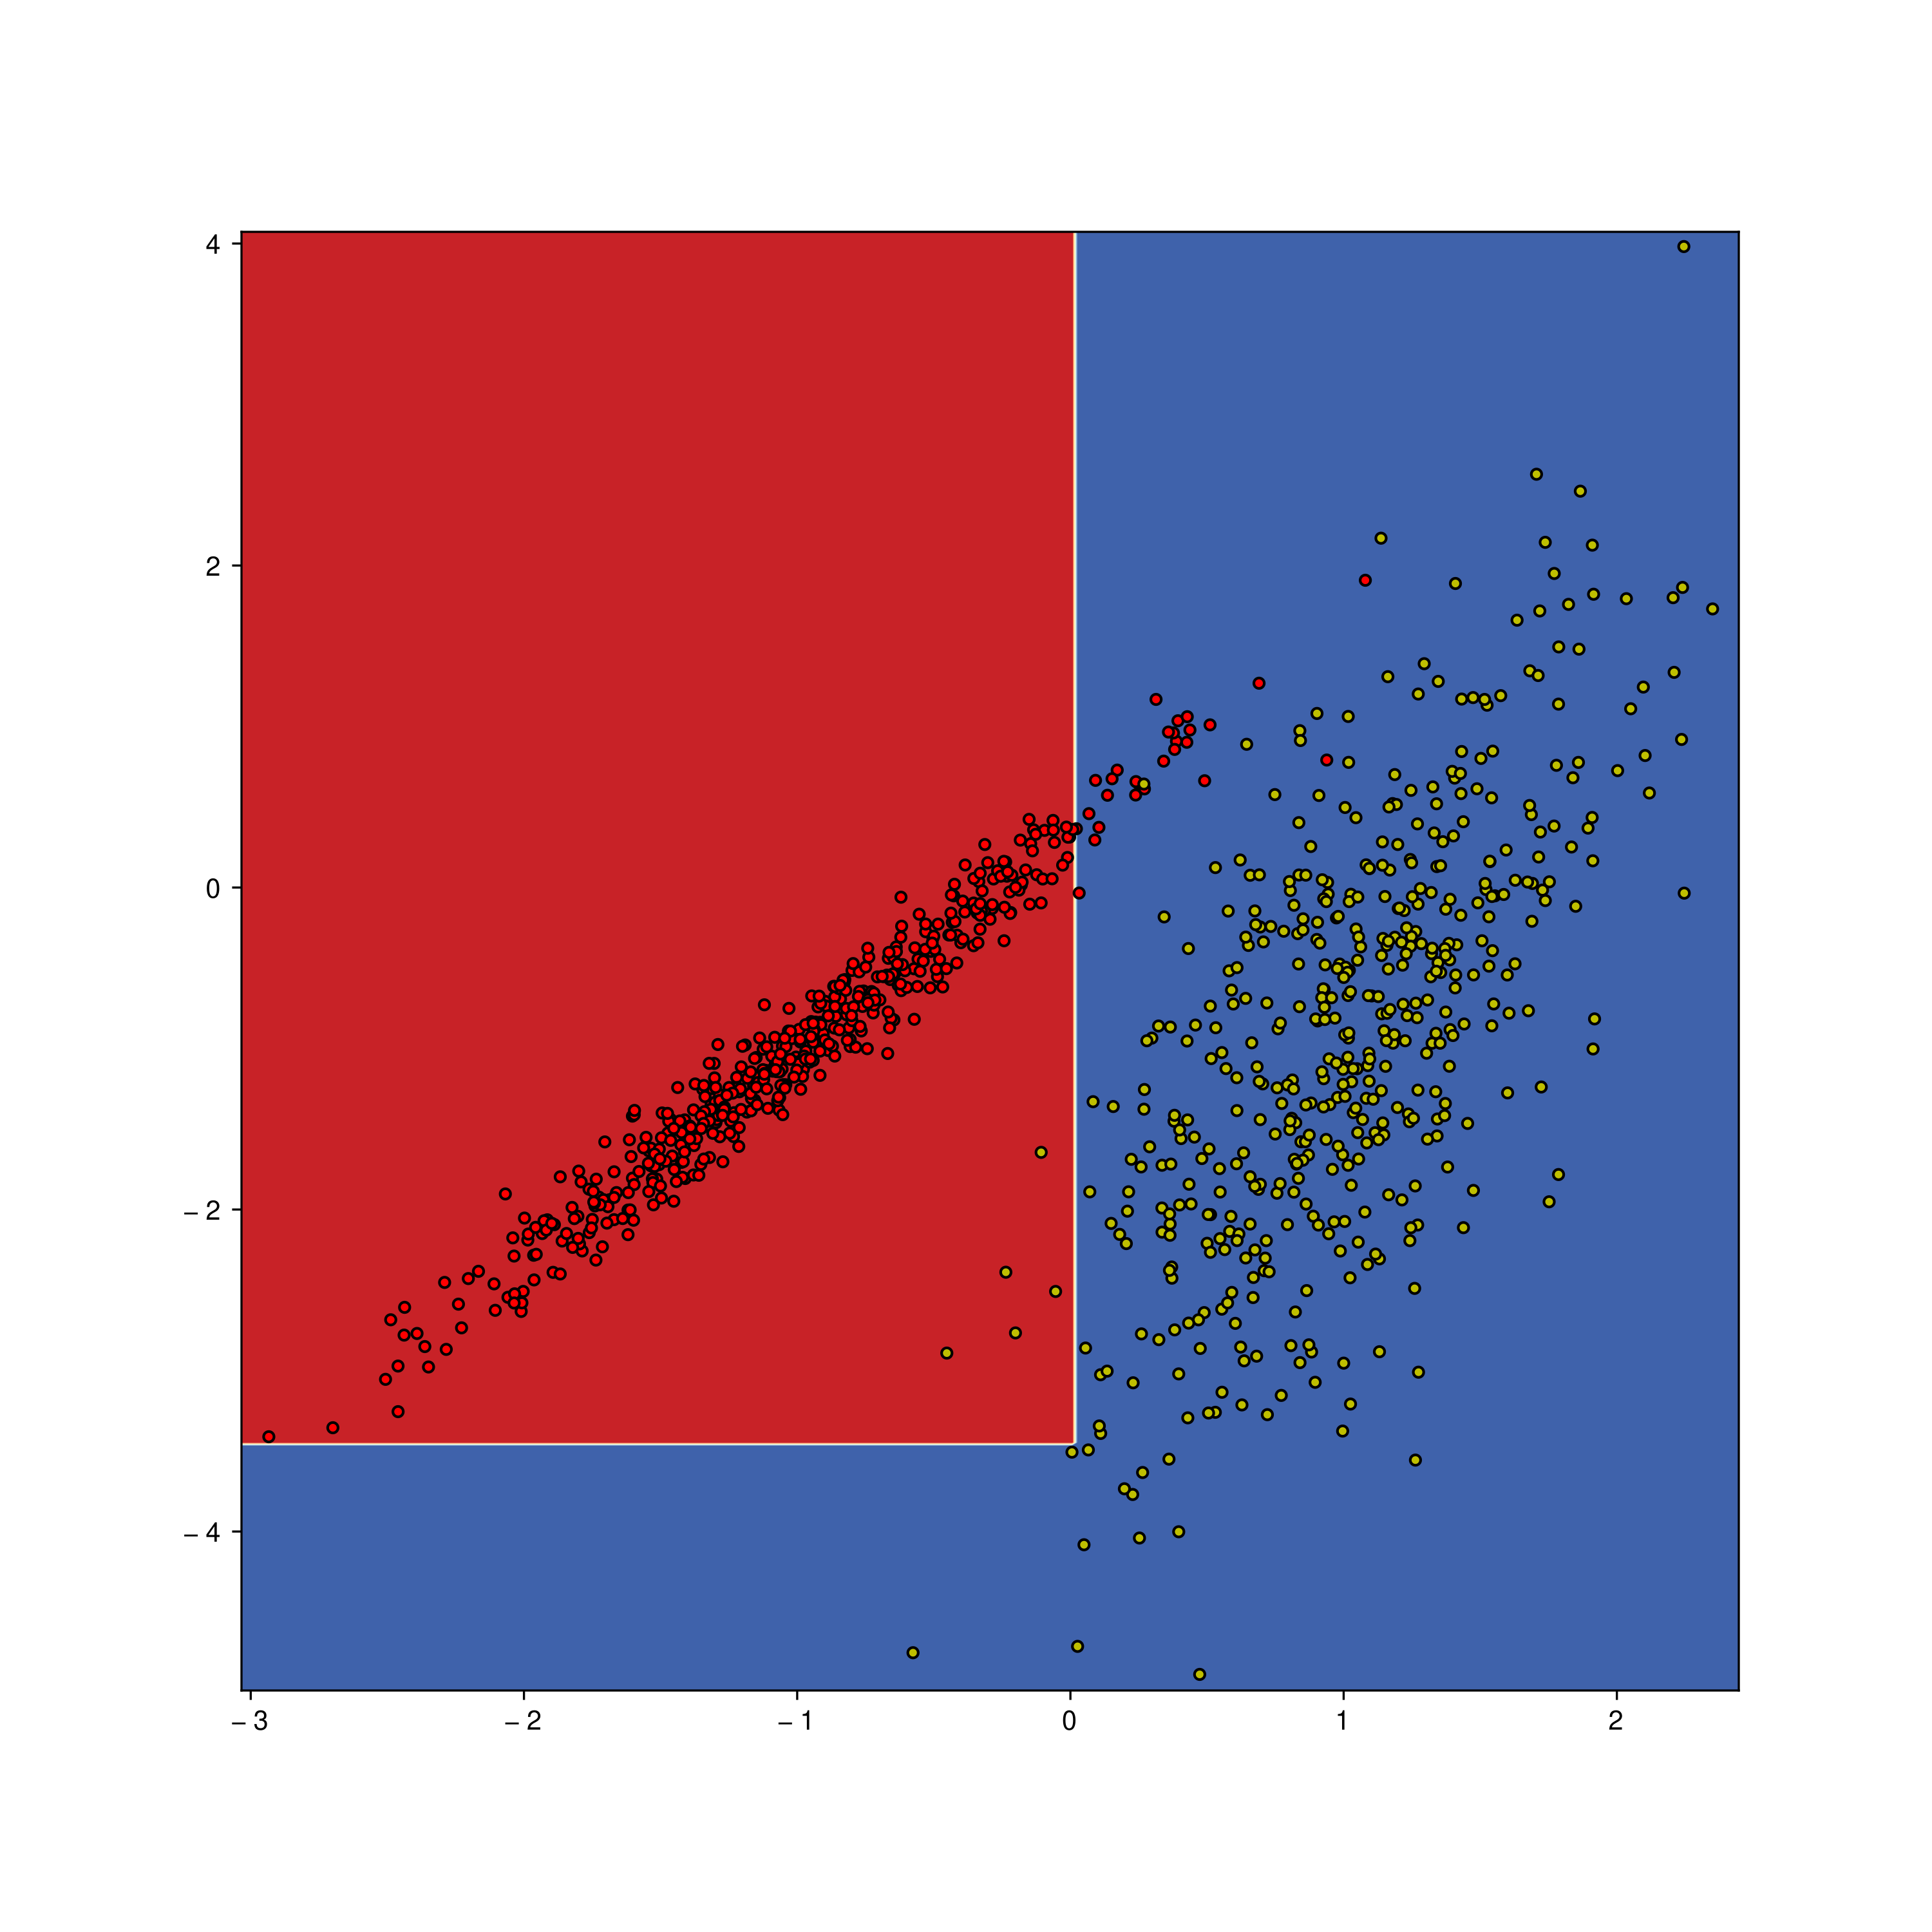
\includegraphics[width=0.7\textheight]{2gi.png}
		\end{figure}
	}
	
	\only<3>{
		\begin{figure}
			\centering
			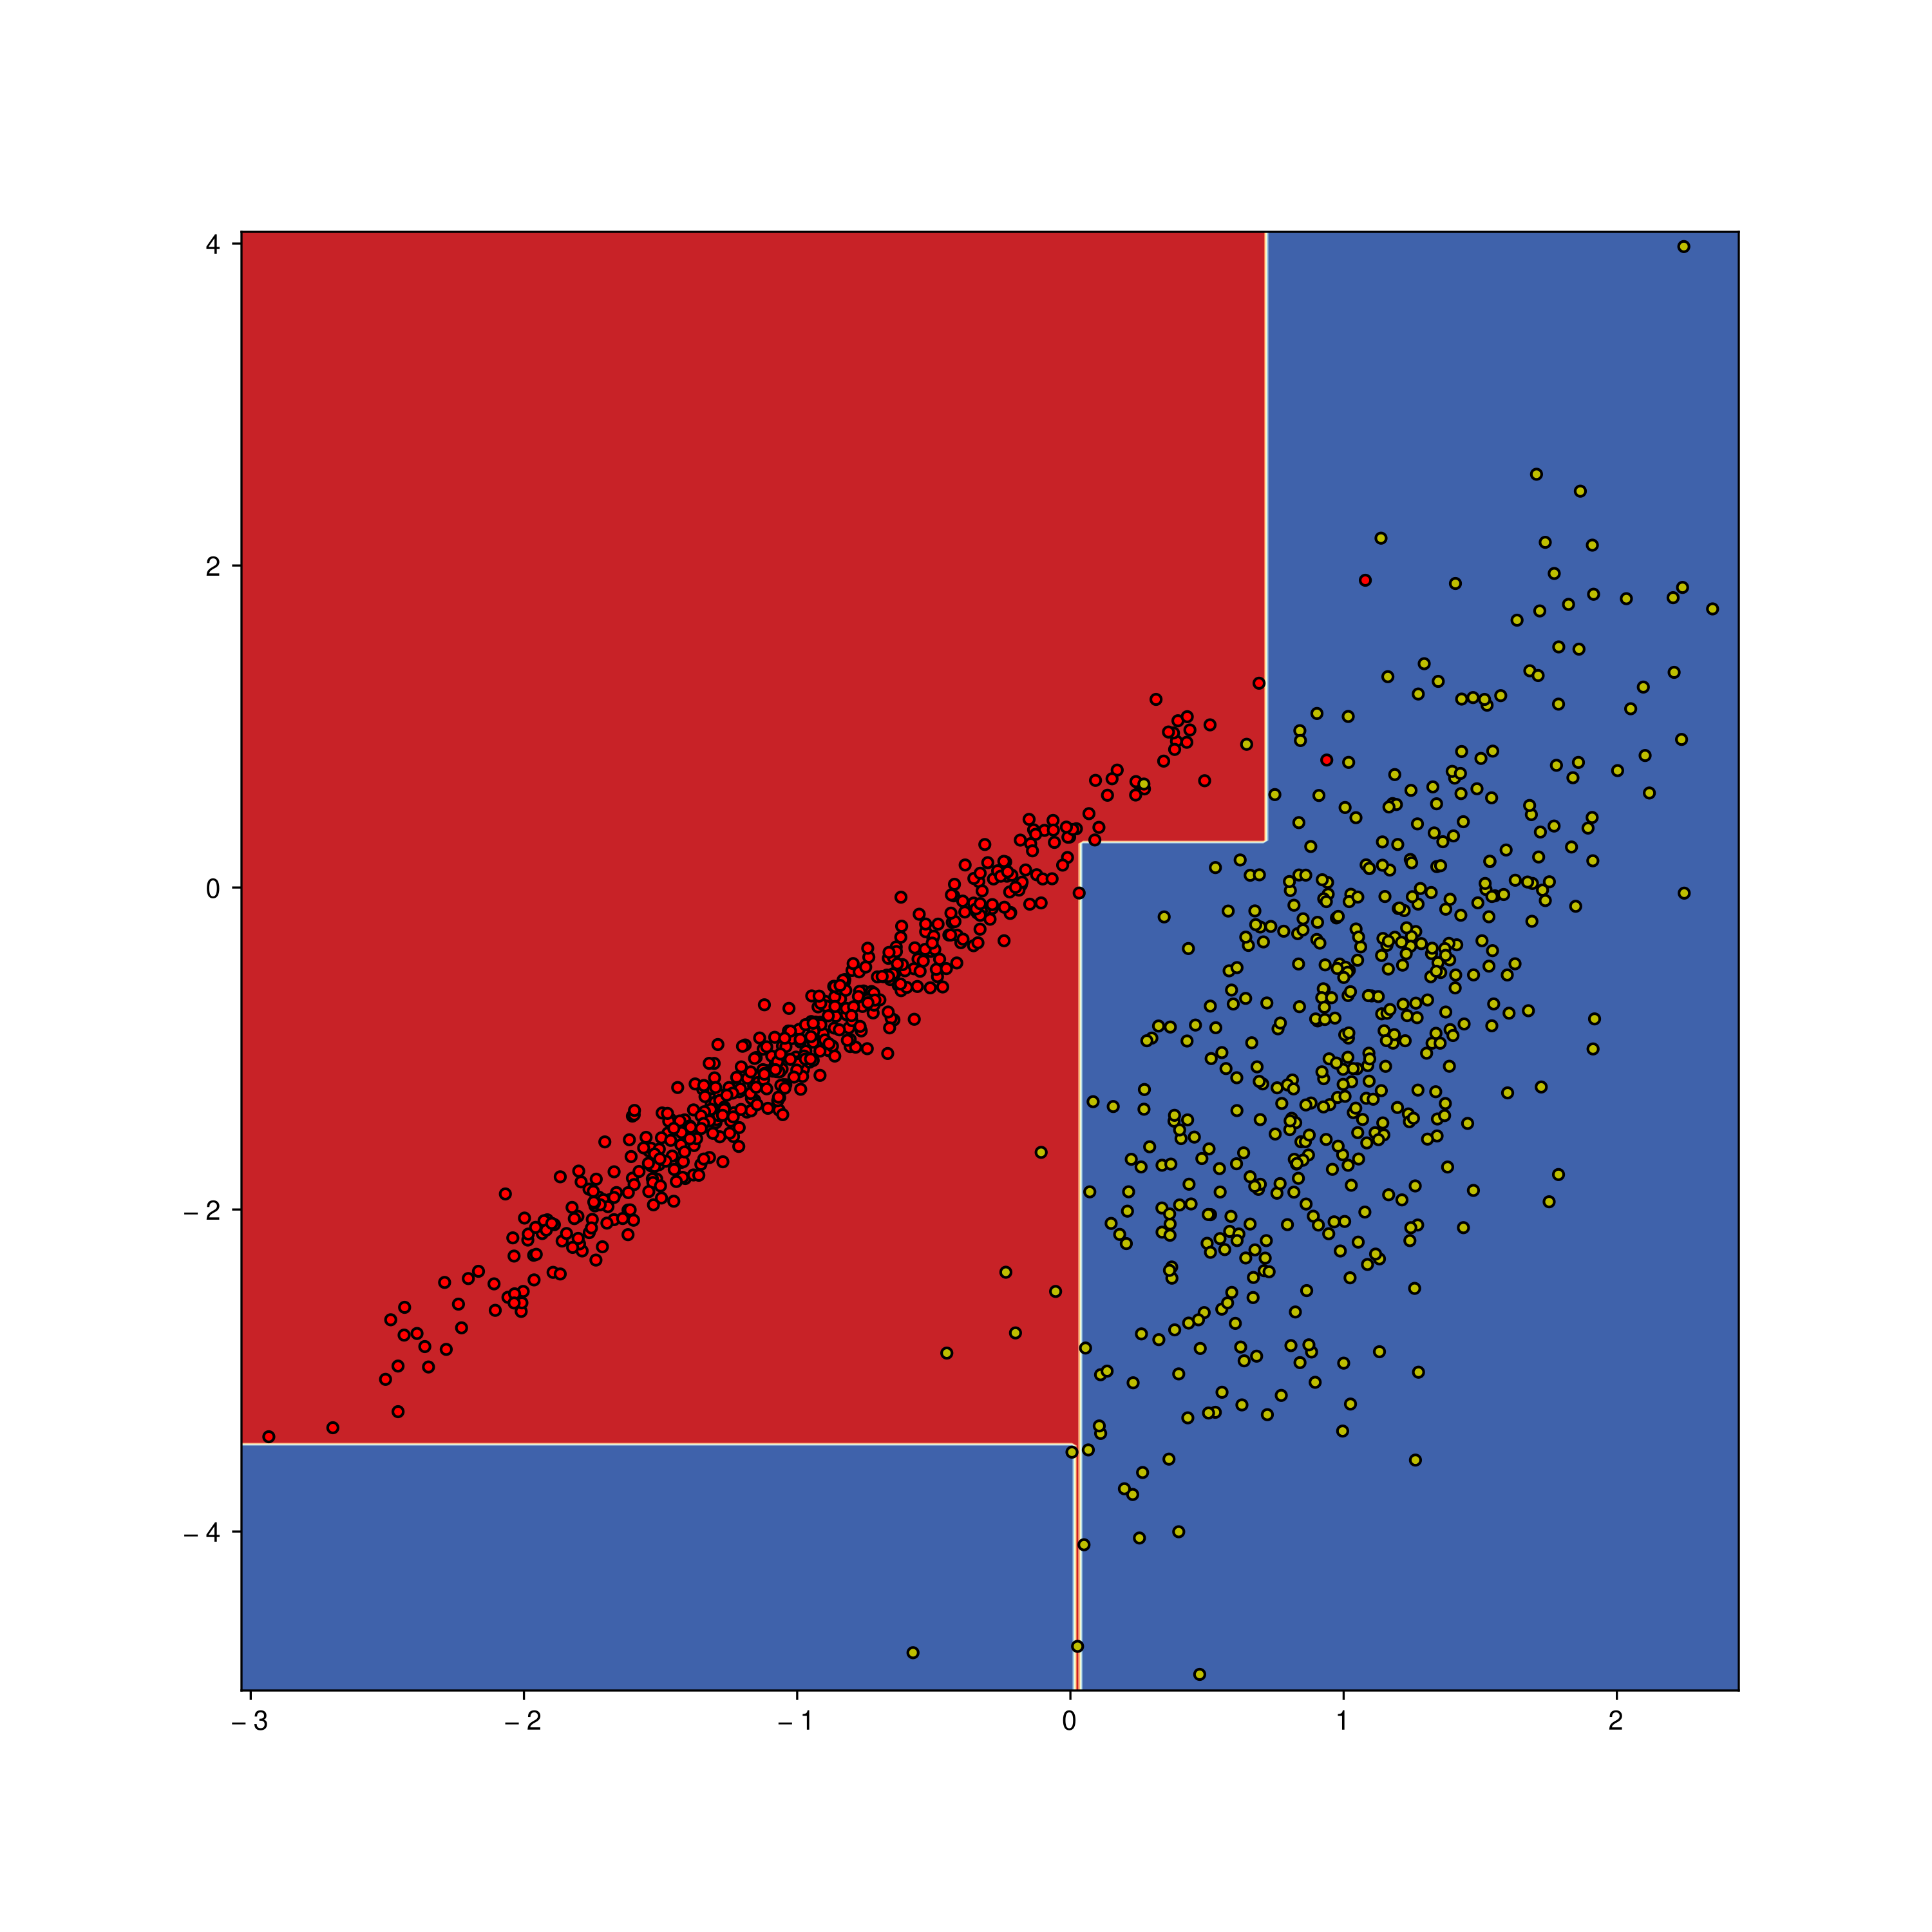
\includegraphics[width=0.7\textheight]{3gi.png}
		\end{figure}
	}
	
	\only<4>{
		\begin{figure}
			\centering
			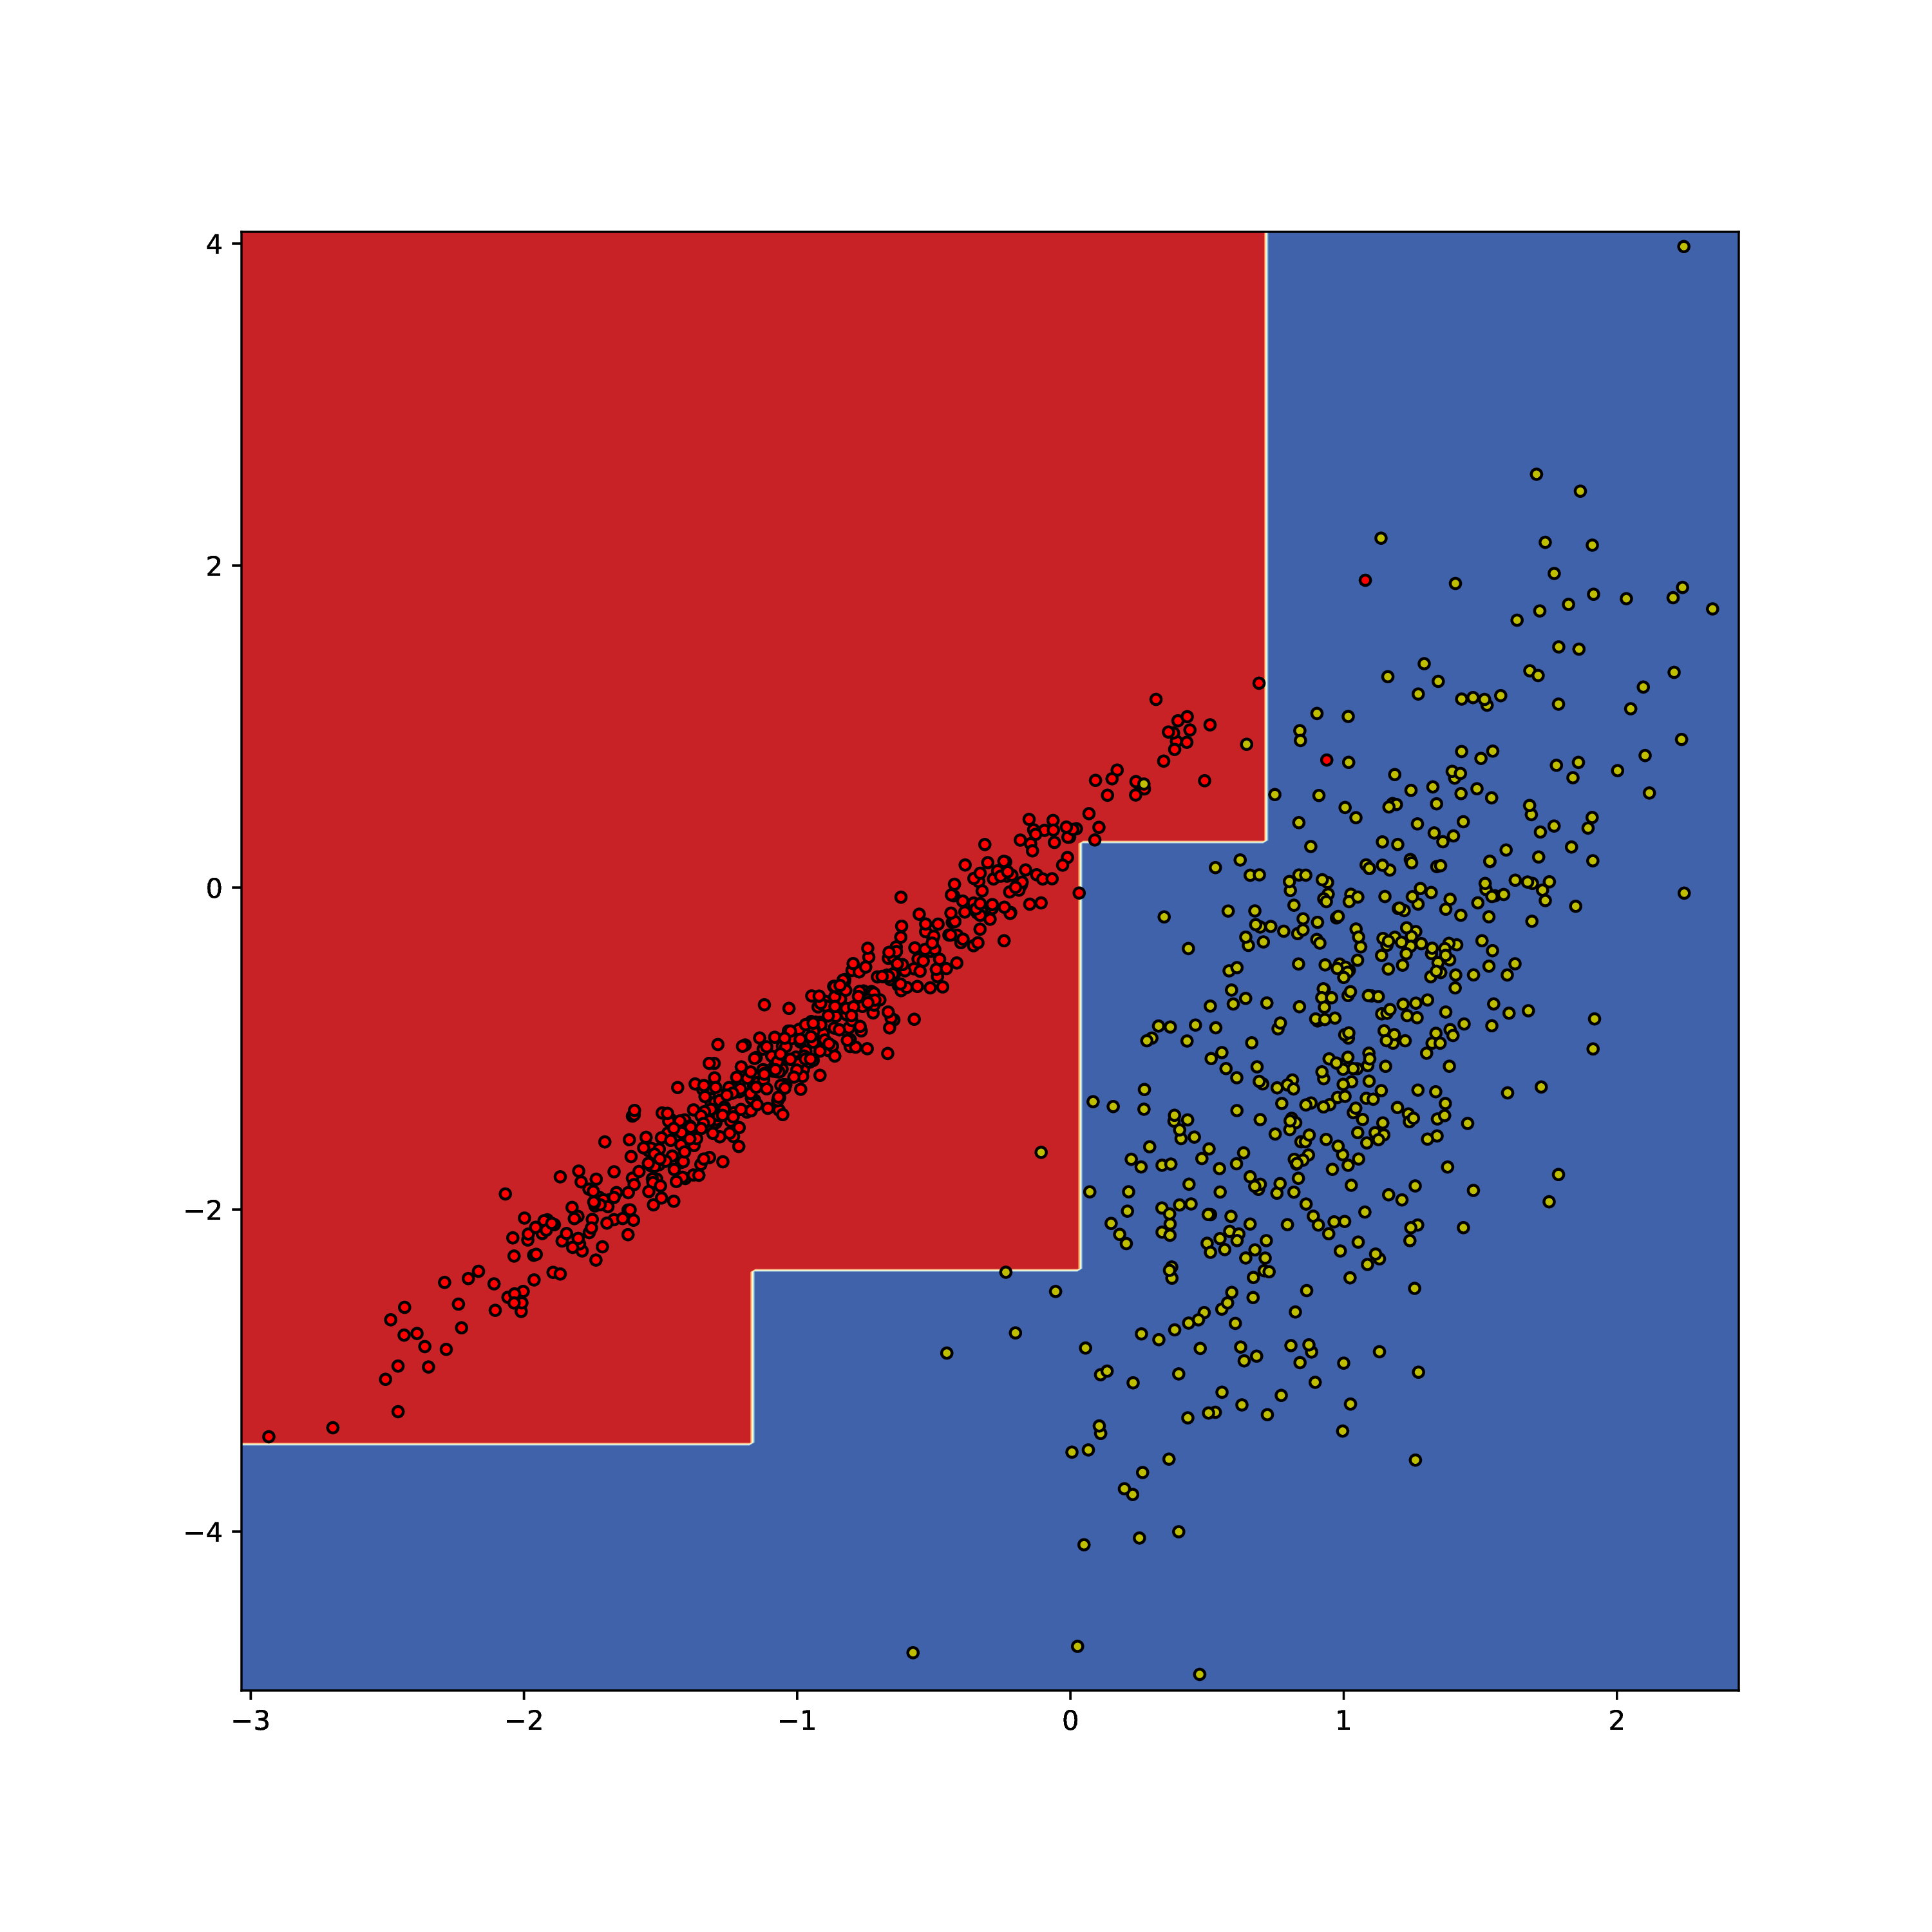
\includegraphics[width=0.7\textheight]{4gi.png}
		\end{figure}
	}
\end{column}

\begin{column}{0.5\textwidth}
	
	\only<1>{
	\begin{figure}
		\centering
		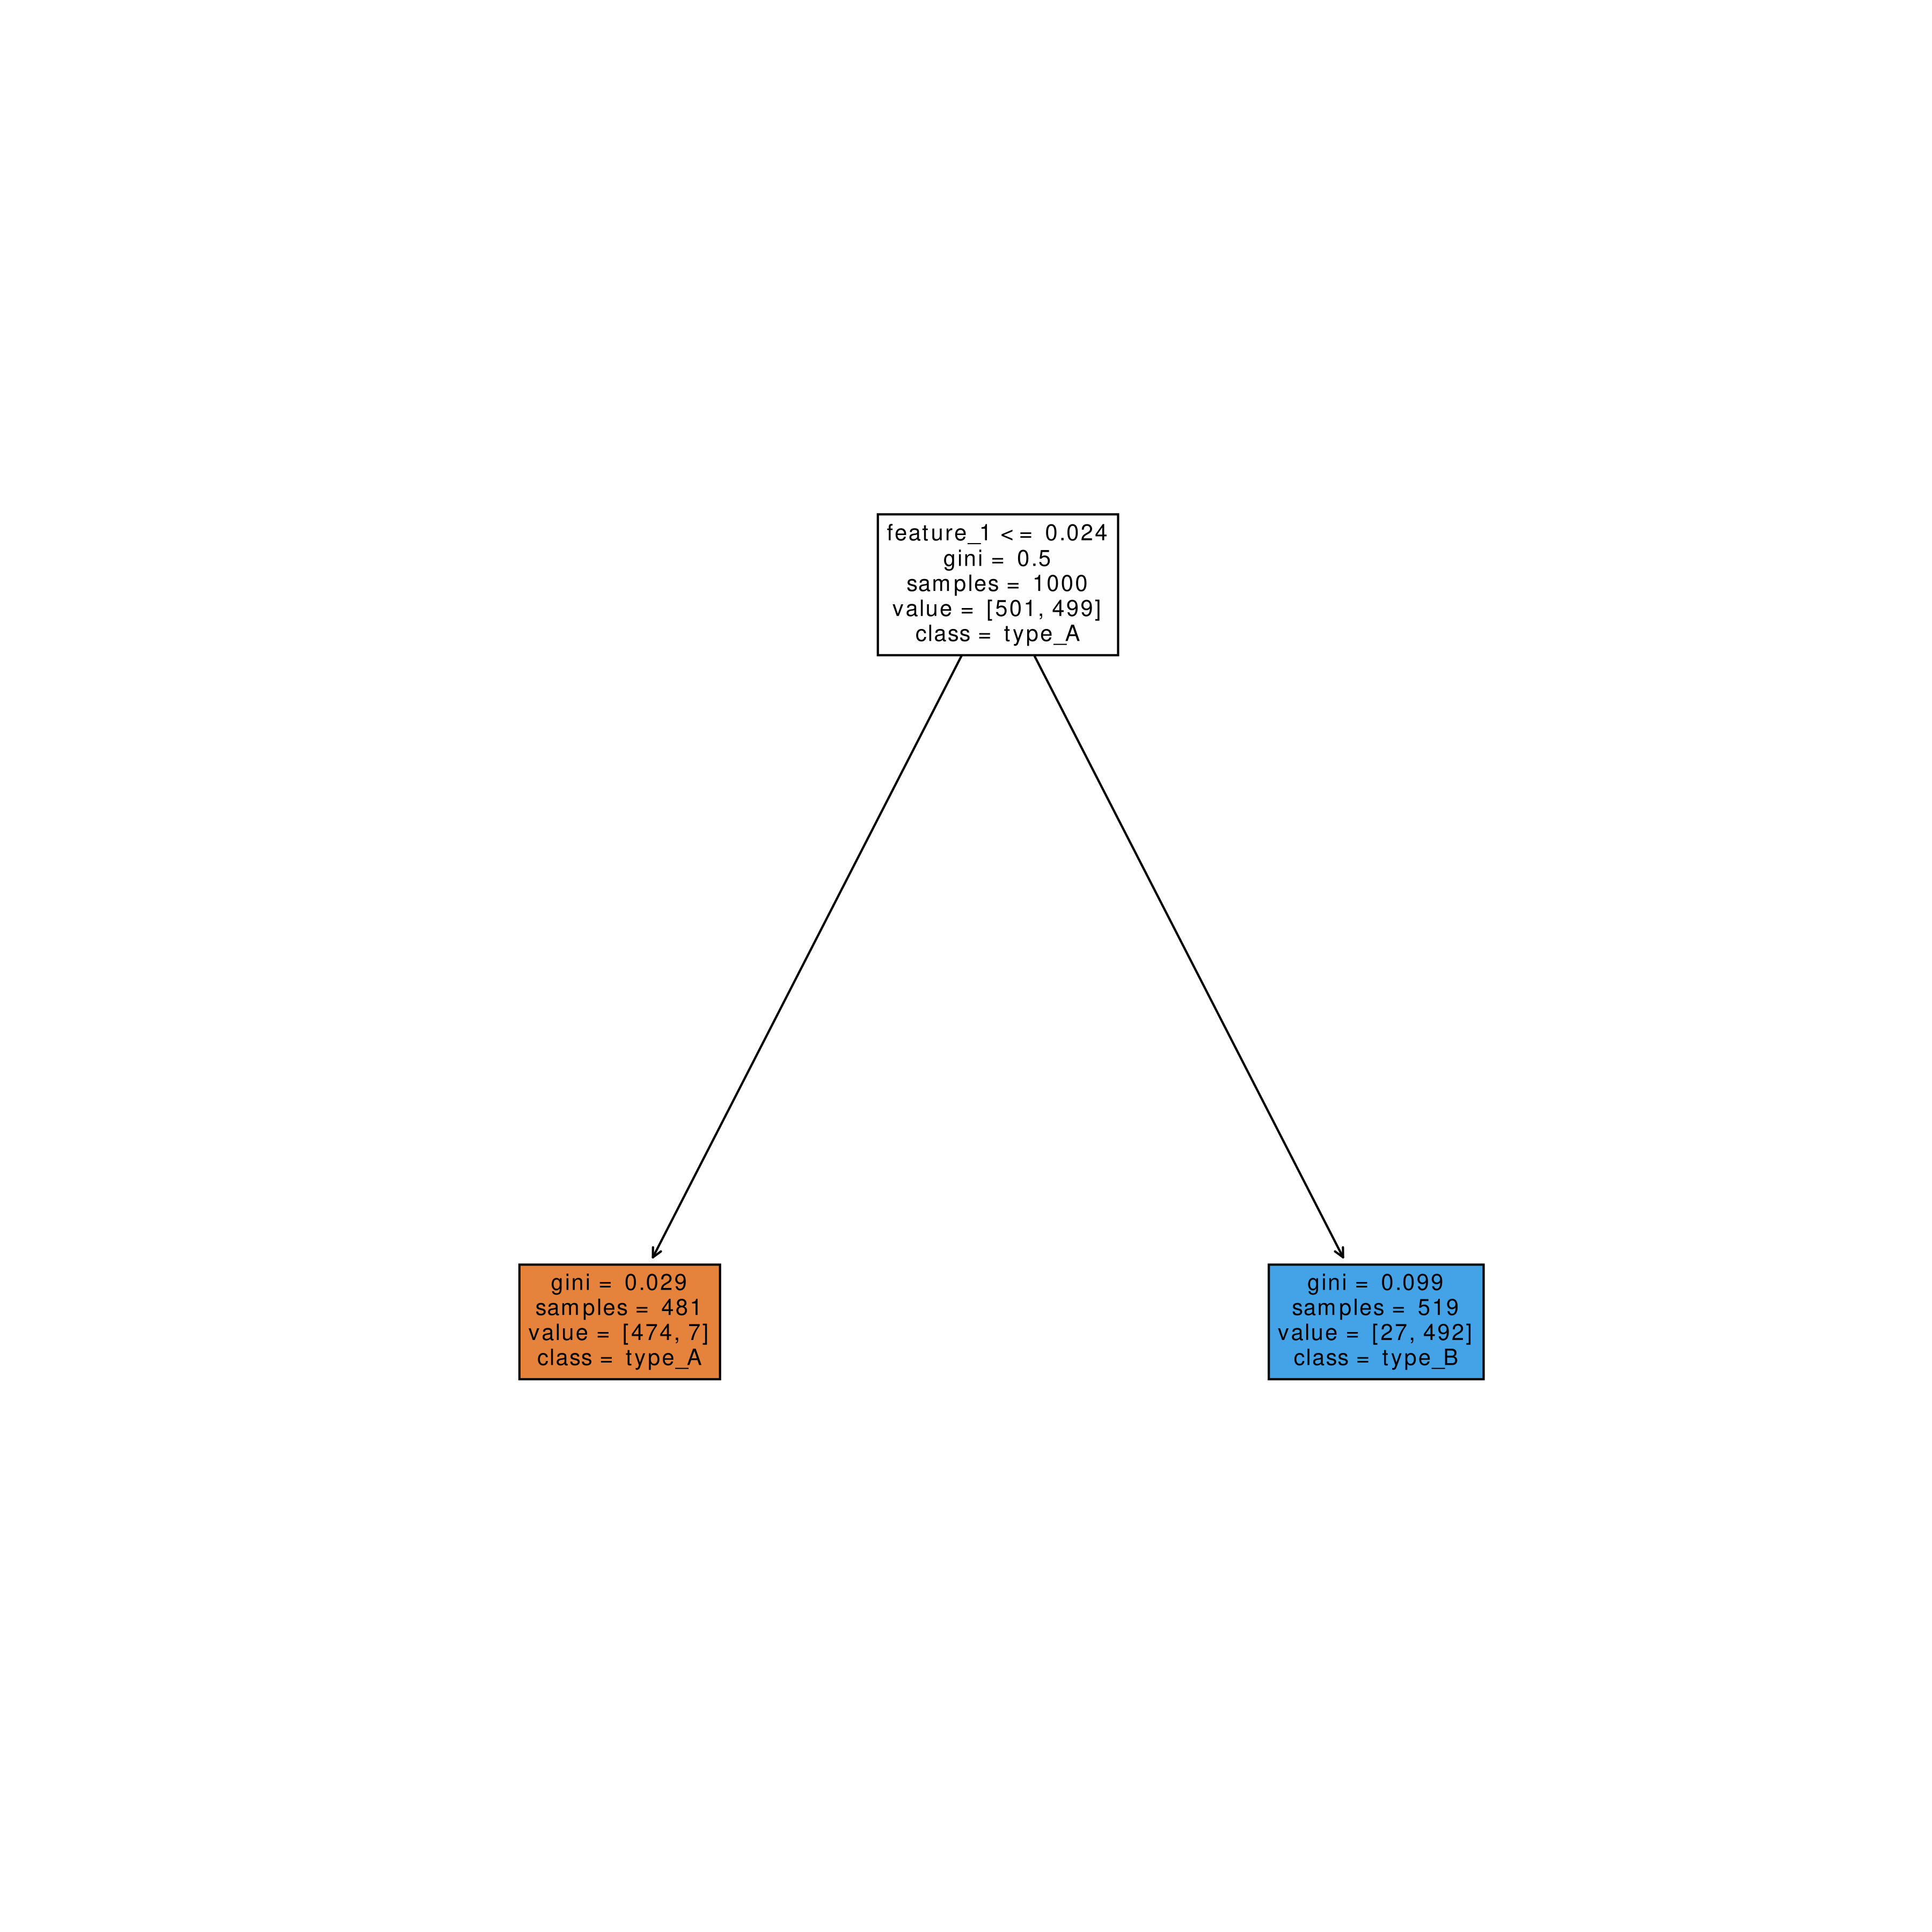
\includegraphics[width=0.9\textheight]{1tree.png}
	\end{figure}
}

	\only<2>{
	\begin{figure}
		\centering
		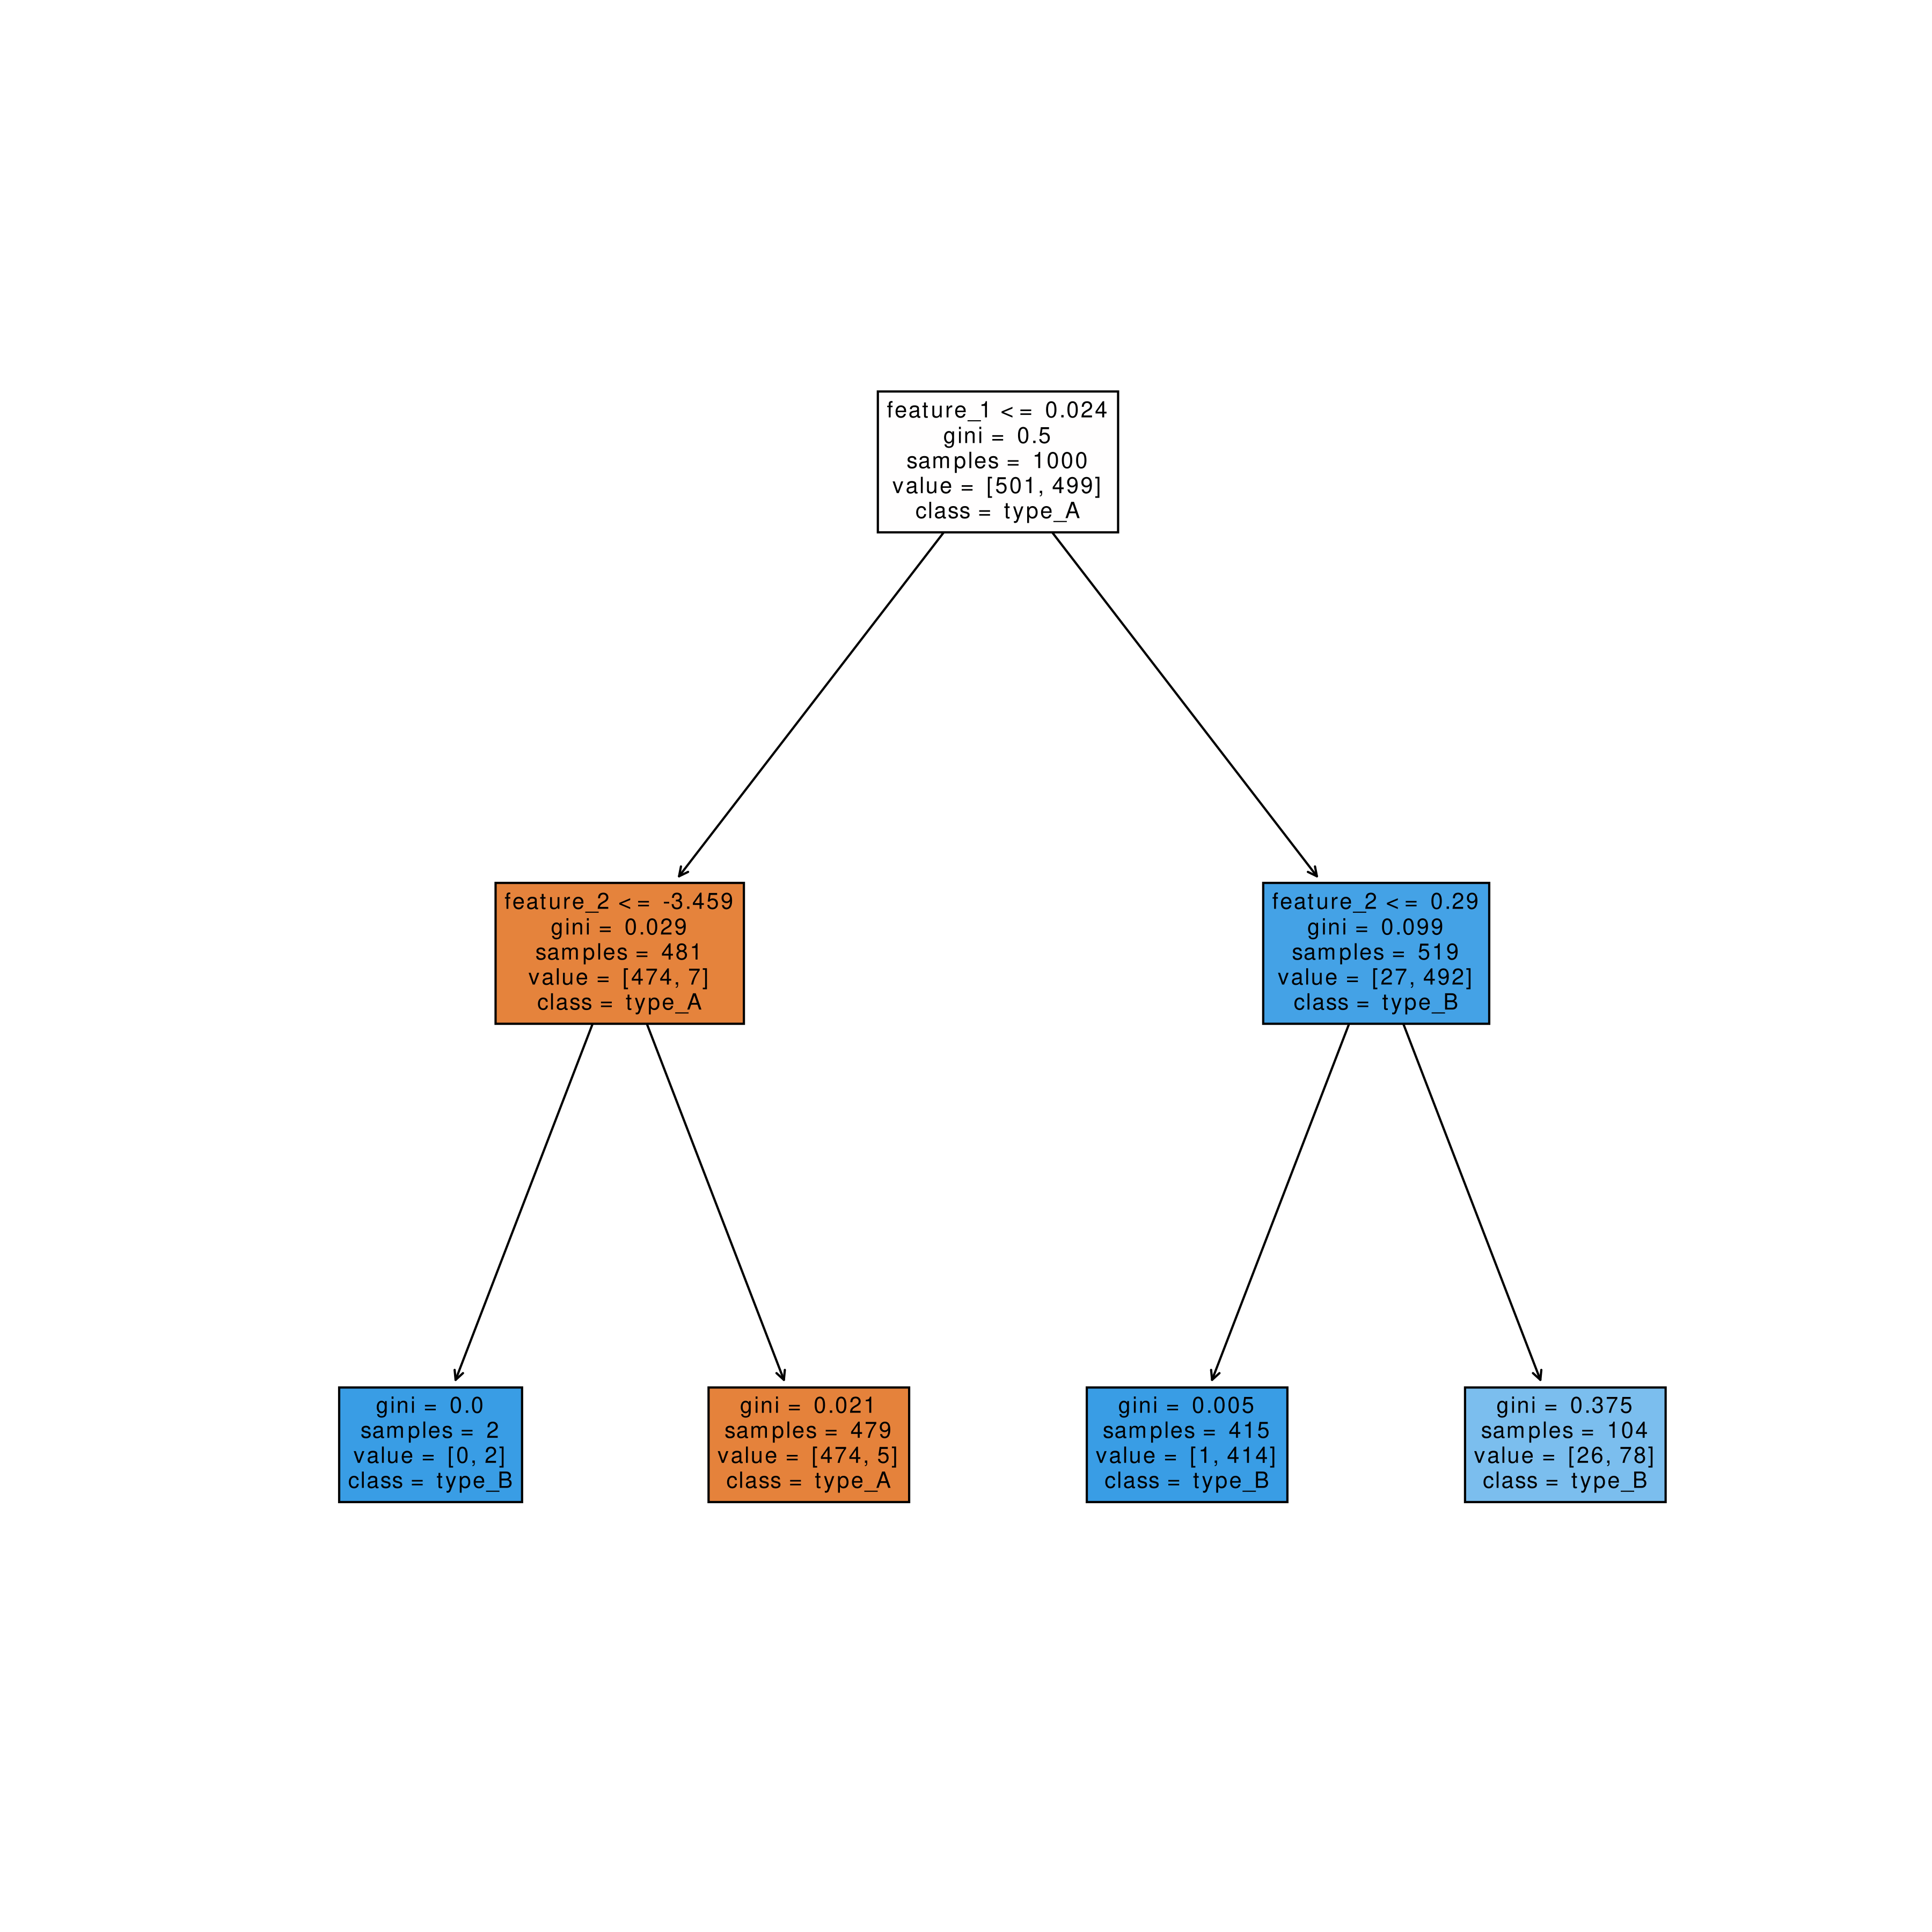
\includegraphics[width=0.9\textheight]{2tree.png}
	\end{figure}
}

	\only<3>{
	\begin{figure}
		\centering
		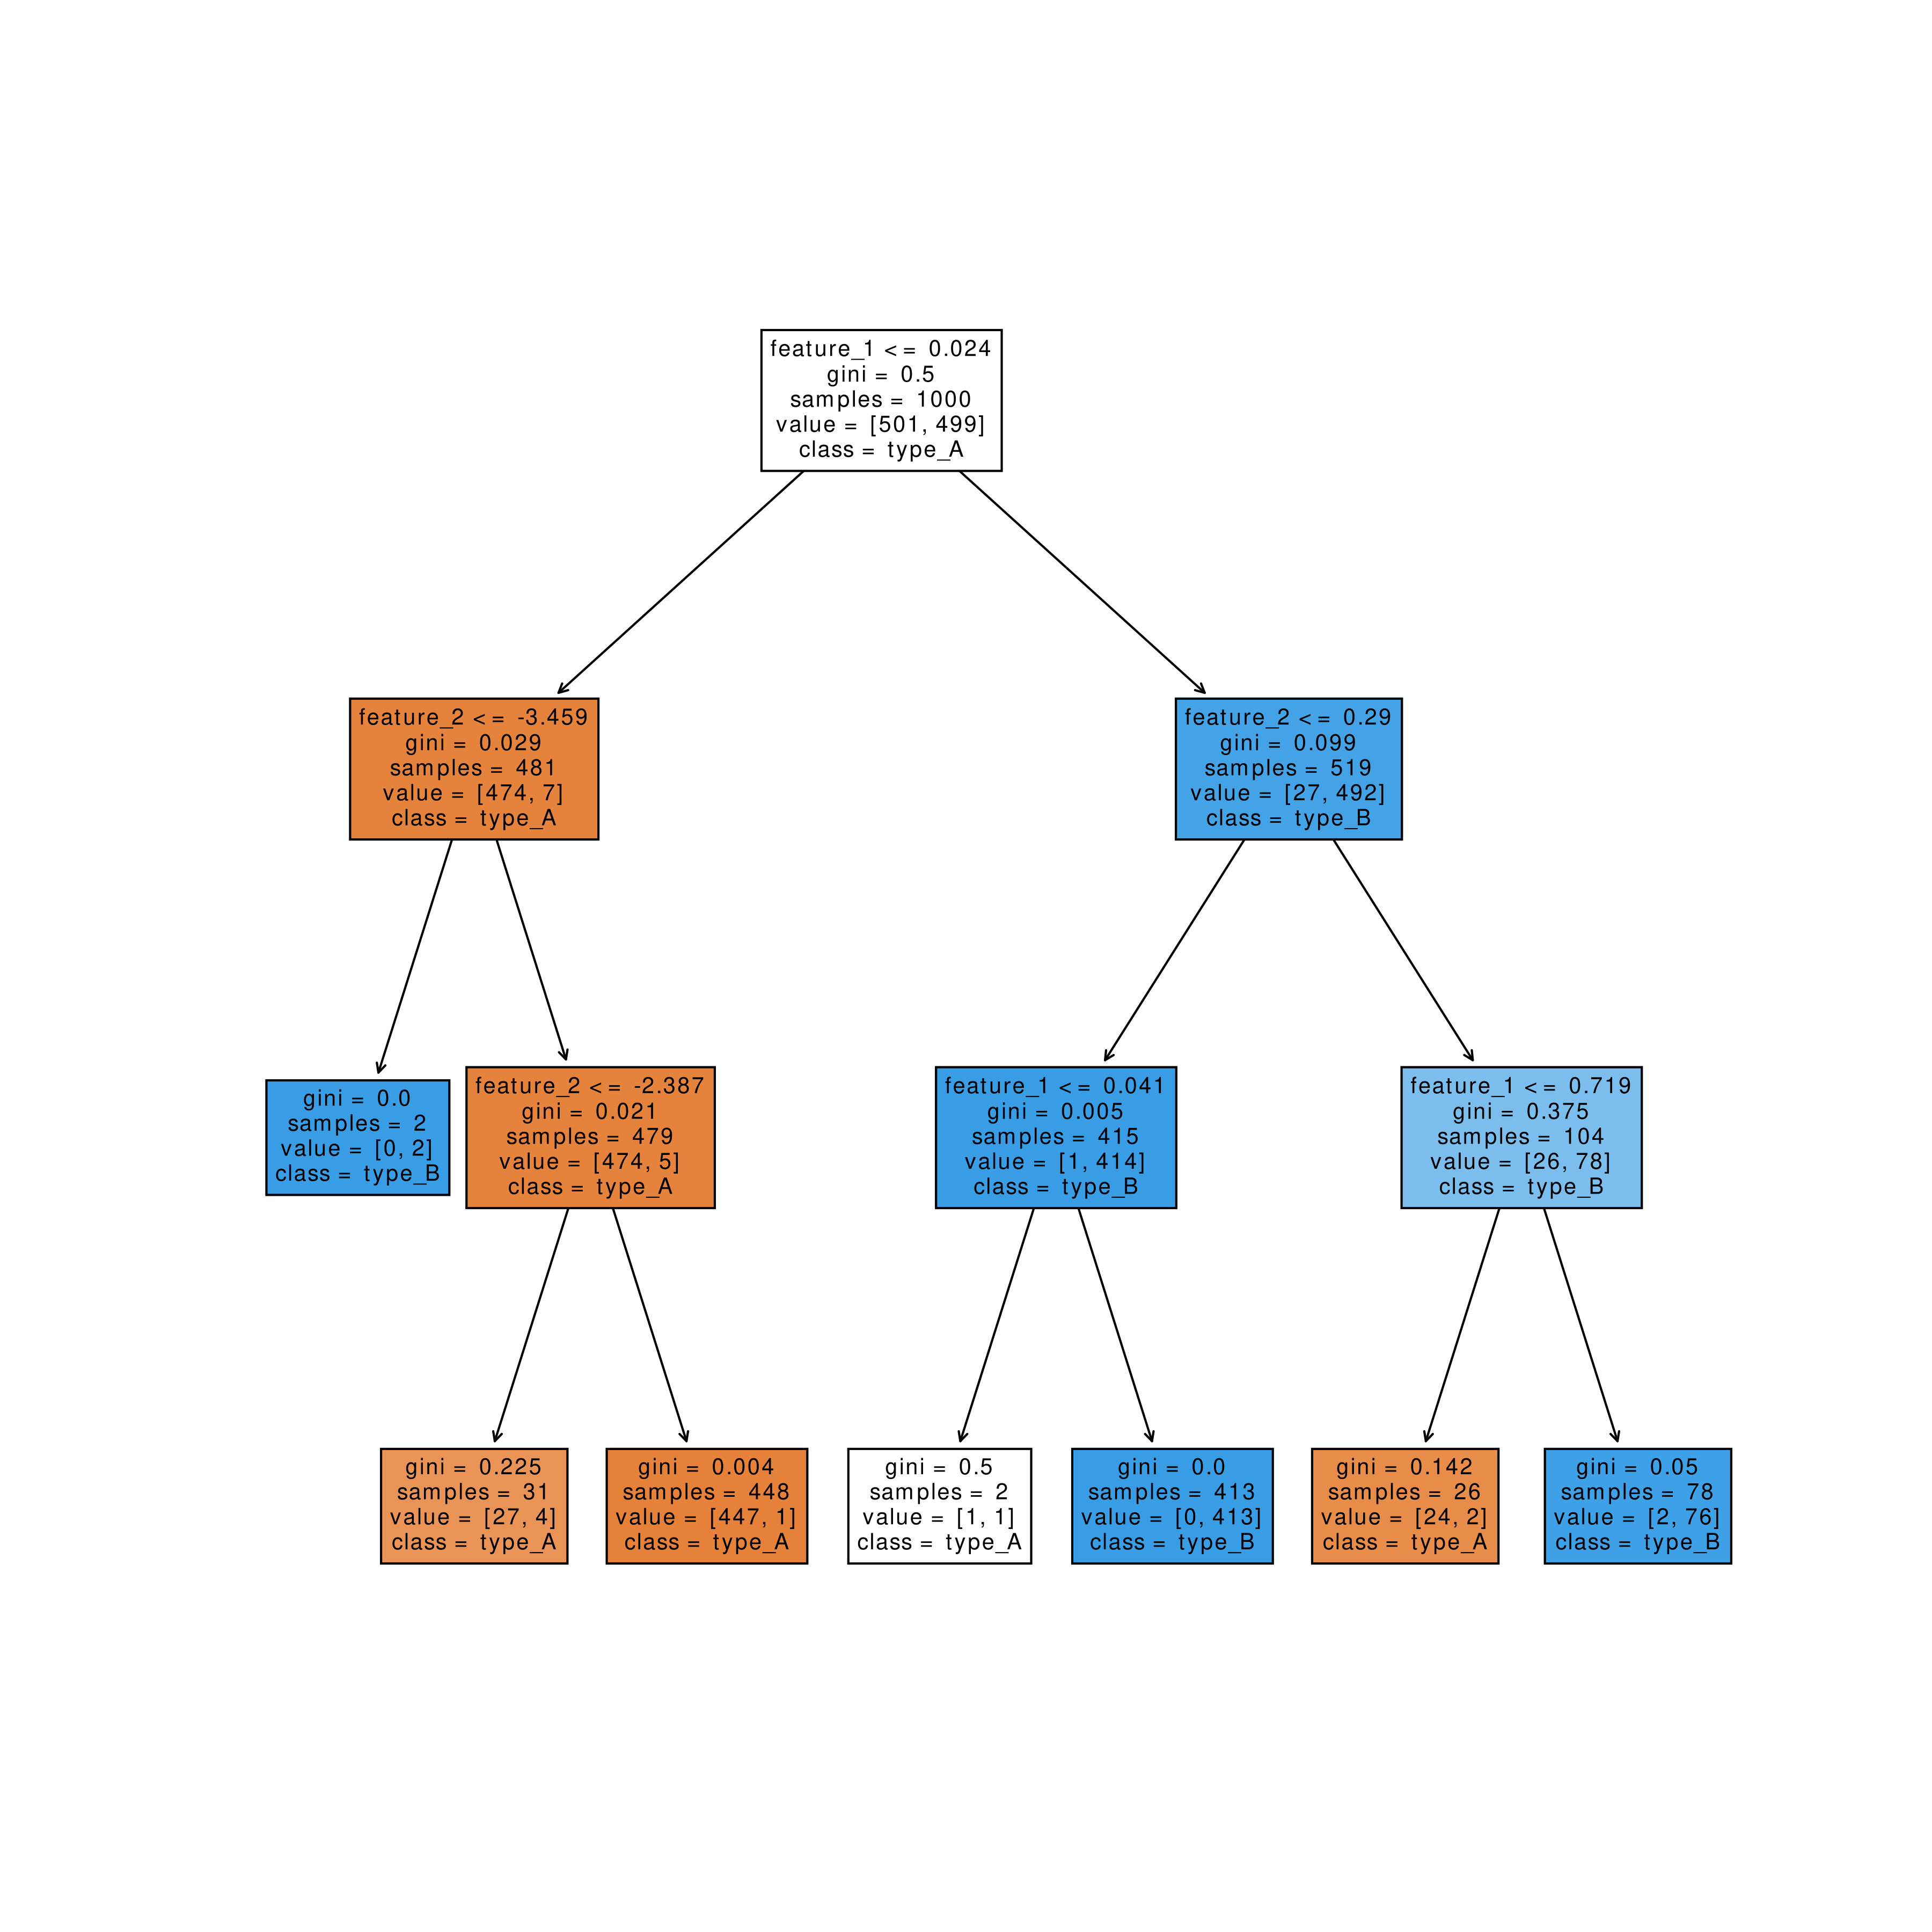
\includegraphics[width=0.9\textheight]{3tree.png}
	\end{figure}
}

	\only<4>{
	\begin{figure}
		\centering
		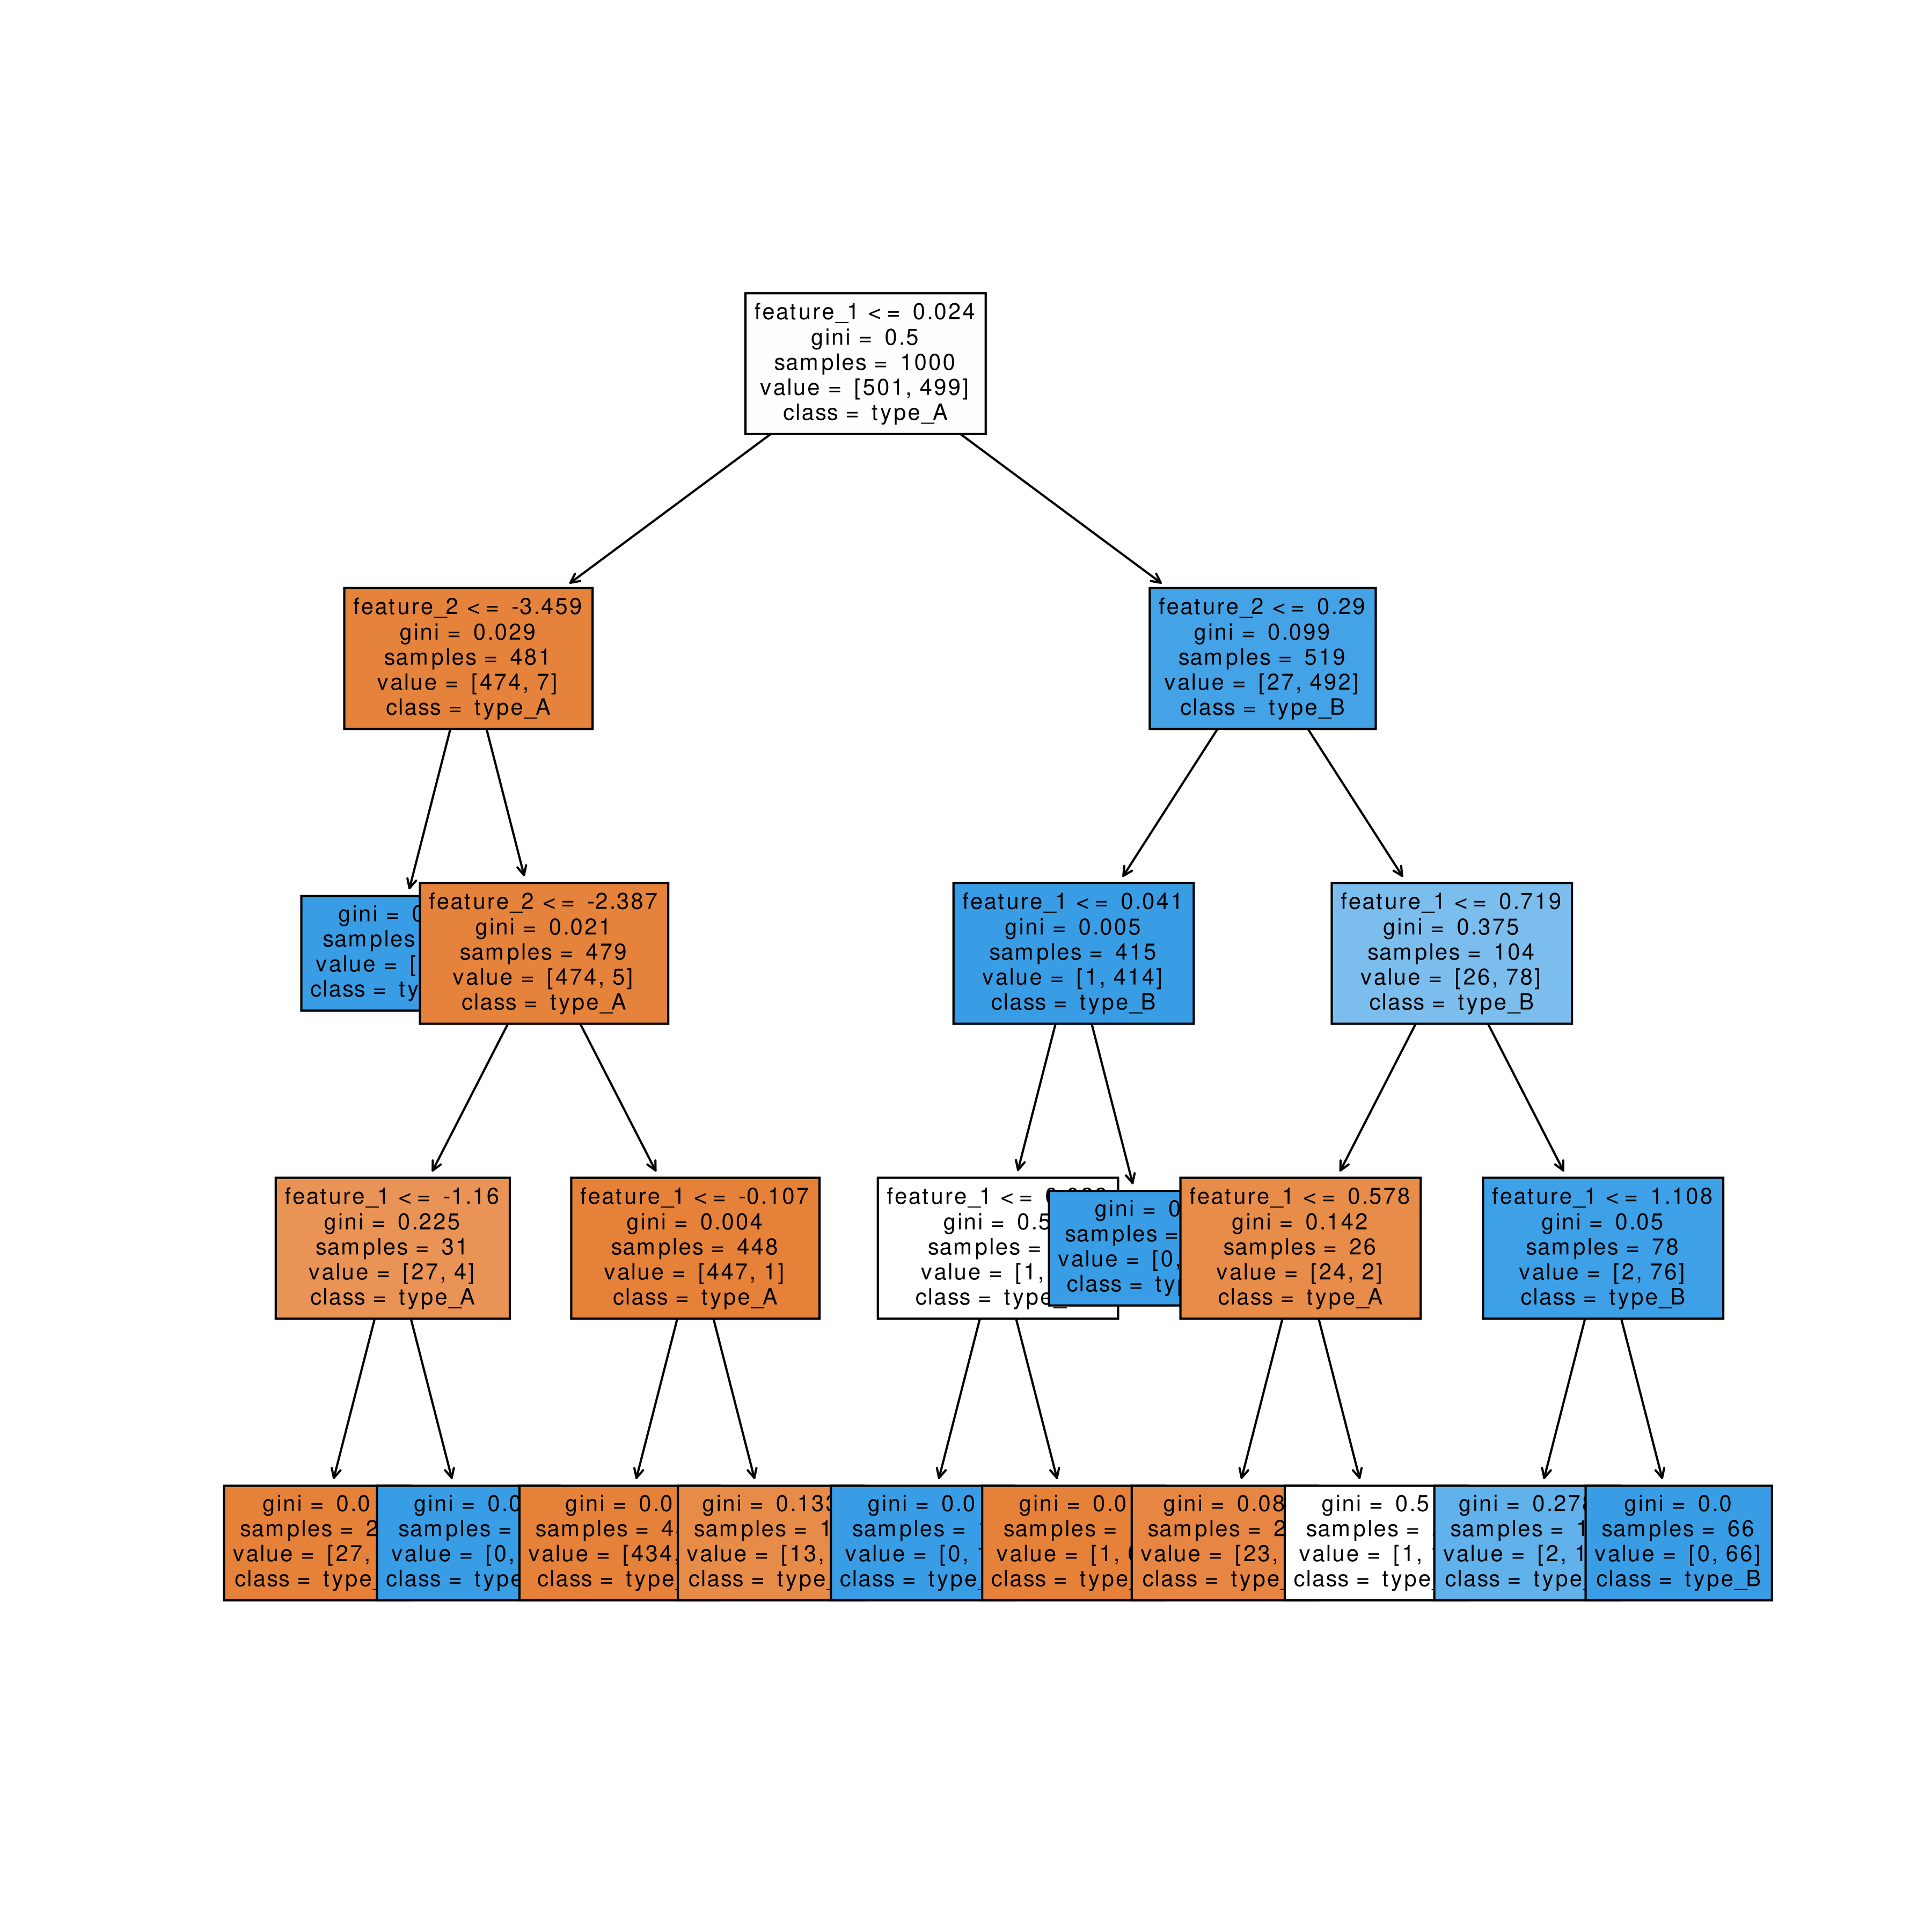
\includegraphics[width=0.9\textheight]{4tree.png}
	\end{figure}
}
\end{column}
\end{columns}


\begin{textblock*}{0.45\paperwidth}(0.7\paperwidth,0.1\paperheight)
	\footnotesize
	\textcolor{Gray}{check out also \href{http://www.r2d3.us/visual-intro-to-machine-learning-part-1/}{\underline{these}} visuals}
\end{textblock*}


\end{frame}

%------------------------------------------------
%------------------------------------------------
\section{Random forest and gradient boosting}
%------------------------------------------------
%------------------------------------------------

\begin{frame}[plain]
\centering
\huge
%\begin{textblock*}{0.3\paperwidth}(0.25\paperwidth,0.3\paperheight)
\centering
\vspace{0.1\paperheight}
\begin{tcolorbox}[colframe=white, colback=mygrey, width=0.62\paperwidth,
arc=2.mm, boxsep=2mm,
box align=center,
halign=center,
valign=center,
]
\insertsection
\end{tcolorbox}
%\end{textblock*}
\transfade[duration=.4]
\end{frame}

%------------------------------------------------

\subsection{what's next after decision trees?}
\begin{frame}
\myframetitle{0.45\paperwidth}{0.04\paperwidth}{\insertsection}
\myframesubtitle{0.47\paperwidth}{\insertsubsection}

\vspace{0.15\paperheight}
\begin{columns}
\column{0.5\textwidth}
\centering
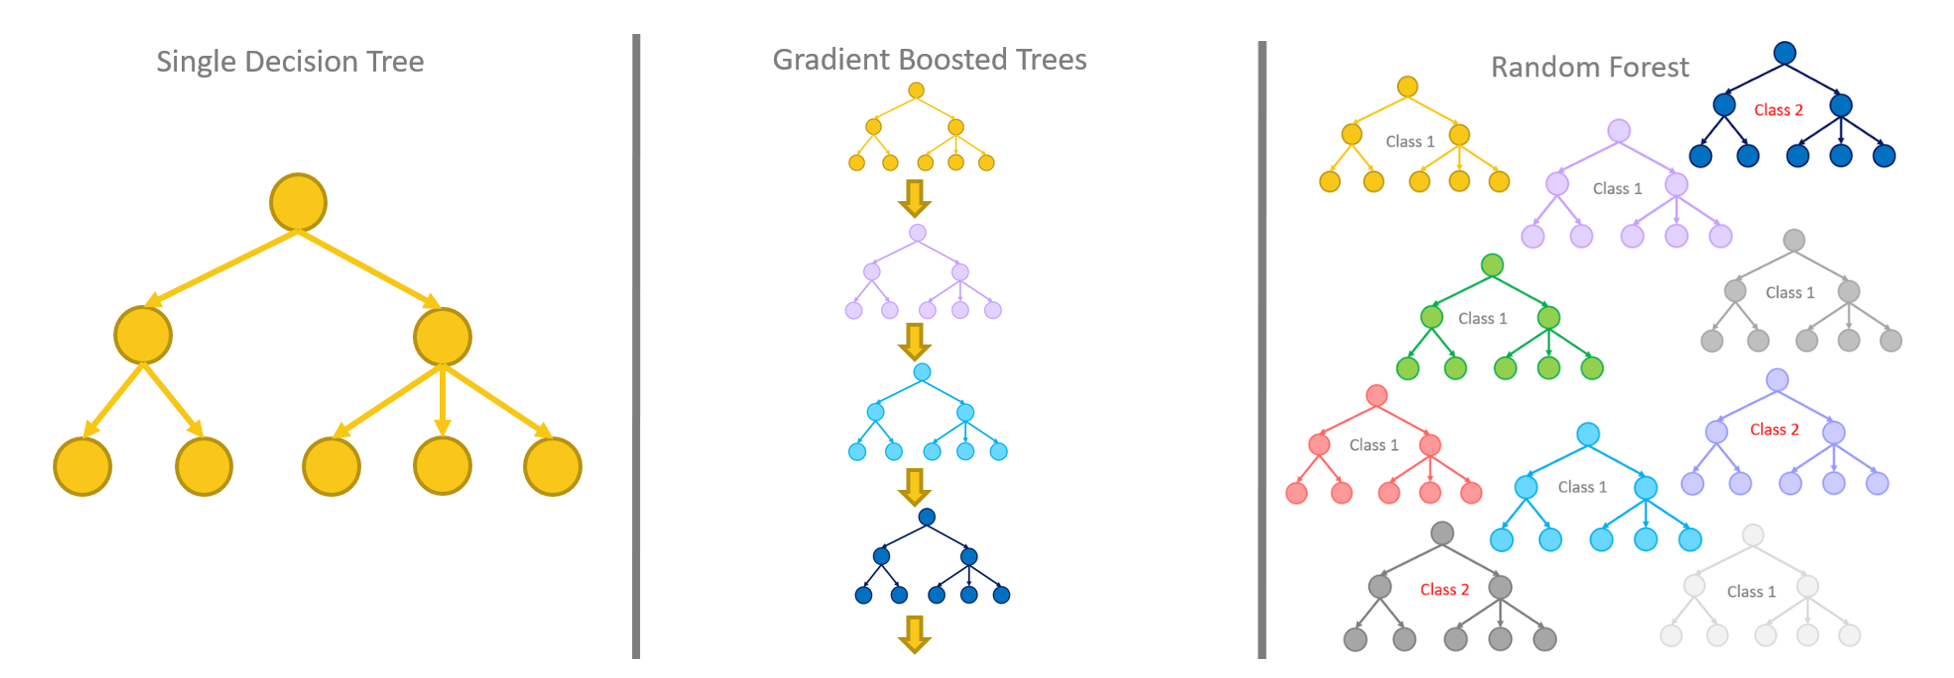
\includegraphics[width=1.15\textwidth]{trees.png}

\column{0.5\textwidth}
\centering
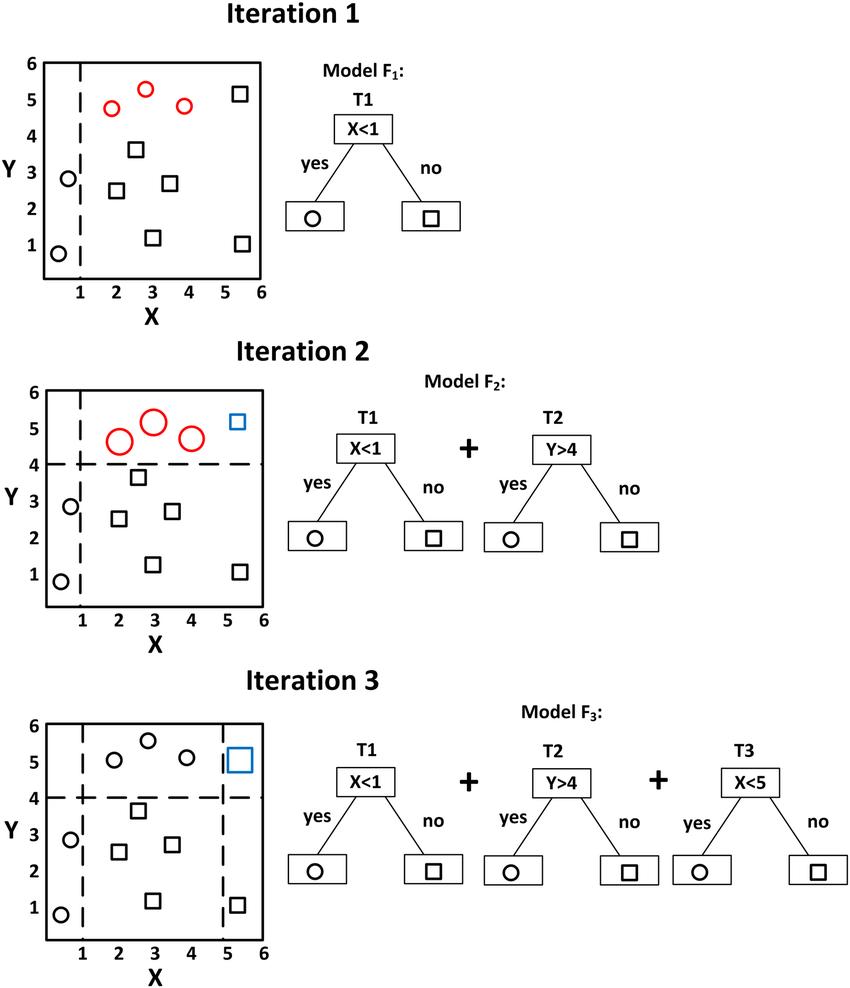
\includegraphics[width=0.8\textwidth]{gradient_boosting.png}
\end{columns}

\end{frame}

\end{document}
